% !Mode:: "TeX:UTF-8"

\chapter{全局语义轨迹压缩算法}
\label{chapter:main1}

理论上,我们可以每秒为单位来记录移动物体的轨迹信息。但是,这将会耗费大量诸如存储空间以及通信资源,并在计算上产生不小的开销。实际上,许多应用场景不要求非常精准的位置信息。为此,研究者们提出了轨迹数据压缩的算法来将海量的轨迹压缩至可接受的开销范围内。本章中我们将提出一种全新的轨迹压缩算法,来克服上一章提到的传统压缩算法的缺点。


\section{问题描述}
\label{sec:start}
就如同上一章中回顾的那样,主流的轨迹压缩有两种:将轨迹视为线条组合的传统轨迹压缩方法和加入各种额外信息的语义轨迹压缩法。后者很好的考虑了城市中例如POI或者道路网的约束,从而在压缩结果中保留有用的语义信息。然而有一个问题始终无法得到解决:轨迹压缩的性能始终被语义信息的质量所决定:如果道路网部分缺失、或者POI信息不全,那么基于这些信息的轨迹表征方法将大大收到影响。

本文将介绍一种基于同步聚类算法的多粒度轨迹压缩算法,\CascadeSync,这为轨迹压缩提供了一种新思路。与独立提取每个轨迹中的关键点的传统方法不同,\CascadeSync是一种旨在找到允许表示所有原始轨迹点(即全局结构信息)的重要区域的模型。这些感兴趣的区域(Region of Interest, ROI)是通过基于同步的聚类模型聚合周围的数据点而形成的。在动态的同步聚类算法下,轨迹数据中的这些GPS点可以从细粒度级别到粗粒度级别聚类。利用导出的ROI,轨迹数据可以表示为一组基于ROI的多分辨率网络。另外,如果某些领域知识可以利用,则算法可以将其集成到基于同步的聚类过程中。例如,我们假设有一堆具有语义信息的点,例如地标建筑,道路交叉点或发生重大事件的地方。这些重要点或区域的位置将在基于同步的聚类过程中被固定,并且它们吸引相邻点或区域组合在一起以形成语义聚类,其被称为语义ROI(Semantic ROI)。通过这种方式,GPS点的全局结构信息和语义信息都将被很好地集成到我们的压缩结果中。同时,与传统的基于语义的压缩不同,\CascadeSync在没有语义点或者语义点稀疏或缺失的地方仍然能进行良好的聚类,语义信息只是作为一种补充信息以加强聚类效果。

\pic[!htb]{全局语义压缩算法示意图。(a)80条原始轨迹以及30个固定的语义ROI(蓝色三角)。(b)经过Sync算法自动聚合出的普通ROI以及原本30个语义ROI。(c)用轨迹将两种ROI连接起来,边的颜色和粗细与轨迹数据成正比。(d)普通ROI以及语义ROI的示意图}{width=145mm}{intro_compression}

% \subsection{算法思路简介}
为了展示这一个思路,图\ref{intro_compression}示出了具有80的合成数据集上的玩具示例
轨迹。对于所有这些轨迹,我们假设有30个语义ROI,在图\ref{intro_compression}(a)中表示为蓝色三角形。在压缩的聚类过程期间,具有语义ROI是固定的,并且所有点(包括固定点)相互交互,直到最终相似的点倾向于聚到一起(同步完成)。由于蓝色的语义ROI是固定的,因此在同步过程之后,它们将吸引其相邻的GPS点组合在一起,从而形成更大的语义区域。对于其他GPS点,如果相邻点没有具有语义ROI,则它们自然地组合在一起以形成普通ROI(图\ref{intro_compression}(b))。图\ref{intro_compression}(d)进一步说明了两个得到的ROI:正常ROI和语义ROI。然后,利用这些ROI,每个轨迹可以表示为ROI序列,并且整个轨迹数据被进一步压缩为ROI网络(图\ref{intro_compression}(c))。通过ROI网络,可以很好地保留全局的轨迹移动模式。此外,由于基于同步的聚类的特性,这些ROI可以进一步压缩到更高级别并且产生更紧凑的轨迹表示。基于多分辨率ROI网络表示,可以提取轨迹数据的全局统计数据并且可以促进后续的轨迹挖掘任务(例如,轨迹聚类,分类,模式挖掘和异常值检测)。

\section{基于多层次同步聚类的轨迹压缩算法:CascadeSync}
在本节中,我们将介绍\CascadeSync算法,首先我们介绍算法的相关概念,再阐述如何用同步聚类算法来检测到ROI;之后描述如何将语义ROI融合进这个过程中,让检测出的结果具有语义;最后再阐述如何将这个过程扩展为一个多层次的多粒度压缩算法。


\subsection{概念介绍}
轨迹的定义已经在第\ref{chapter:introduction}章中的(\ref{eq:traj})式中正式的介绍过了。介绍此处将引入误差界的定义,以及语义ROI的概念。

\pic[!htb]{表示误差界的计算示意图。(a)传统轨迹压缩表示;(b)轨迹全局压缩表示。}{width=100mm}{ErrorBound}

传统的轨迹压缩是逐条压缩的,而且是通过去除轨迹中一些采样点实现的。如图\ref{ErrorBound}(a)所示,黑色线条$\left<P_{i-1},P_{i},P_{i+1}\right>$是原始轨迹,而紫色虚线$\left<P_{i-1},P_{i+1}\right>$是压缩后的轨迹。此时蓝色的虚线则为一个表示误差。和传统的轨迹压缩方法不同,\CascadeSync算法由于是全局压缩算法,在压缩后采样点可能便宜之前的位置。如图\ref{ErrorBound}(b)所示,$\left<ROI_{u},ROI_{v}\right>$是压缩后的轨迹表示。此时表示误差为蓝色虚线。为了有正式统一的表示,我们将表示误差界定义如下:

\begin{dingyi}[表示误差界]
给定一条输入轨迹$T$和一个能产生压缩轨迹$T'$的压缩算法$\mathcal{A}$,规定:如果被算法$\mathcal{A}$压缩出来的轨迹$T'$中每一个采样点$P_j' \in T'$都与原轨迹$T$中的$P_j'$的原型点$P_i \in T$的距离满足条件:
\begin{equation}
\label{eq:errorbound}
{distance}\left(P_i,\mathcal{L}(P_j',P_{j+1}')\right) \le \zeta,
\end{equation}
则称算法$\mathcal{A}$的表示误差界为\gls{zeta}。这其中$\mathcal{L}(P_j',P_{j+1}')$是穿过两点$(P_j',P_{j+1}')$的直线。
\end{dingyi}
这种定义很符合直觉,如图\ref{ErrorBound}(b),当新的点$ROI_{u}$与原始点距离$P_i$都不超过误差界$\zeta$,蓝色虚线代表的表示误差自然就会小于$\zeta$。

接下来,我们正式地介绍语义ROI。精确建模轨迹数据中的位置信息在基于地理位置的服务中具有重要意义。由于在许多应用中,由GPS坐标表示的位置不足以支持有效的挖掘任务,我们为了从人类移动性中提取模式,就需要定义活动的位置信息来描述移动对象。有了领域知识之后,可以将轨迹转换为诸如住所,公交车站和学校之类的序列。因此,这使得算法支持涉及语义含义的查询,例如,“给出在某个建筑物钱停留半小时并在8点钟左右通过公交车站的可疑人员”。

到目前为止,有许多算法专门用于自动检测和推断物体的重要位置,比如在轨迹模式挖掘中的工作\citeup{giannotti2007trajectory,liao2007extracting,wang2013mining},在推荐系统中的工作\citeup{tsai2015location,zheng2011recommending,si2017ctf},以及在路径分类中的工作\citeup{lee2008traclass,lv2015measuring}。然而,这些传统的工作的基本思想是简单地将地图分成多个网格或将原始GPS点分组到一些聚类簇中,仍然没办法表示现实中的重要结点。如Richter在其论文\citeup{richter2012semantic}中所述,语义应该明确定义为先验知识。在他们的工作中,重要的城市基础设施比如酒店、大饭点、旅游场所和主要交叉路口都可以被定义为节点;而所有节点可以利用经过这些结点的轨迹扩展为一个网络。我们将这些节点称为语义ROI。通过聚类和地图匹配技术,所有原始GPS点都将被投射到那些语义ROI上。

然而,如我们之前所述,当语义ROI不足以覆盖城市的每个角落时,即先验知识稀疏时,压缩结果中将会被引入大量的误差。而本文可以解决这个缺陷,我们的目标是通过有限的语义信息来进行轨迹压缩。



\subsection{基于同步算法的重要区域检测}
通常,基于同步的聚类算法需要三个关键点来实现:首先是交互参数\gls{epsilon}的定义,其用来指定对象之间的交互范围;第二,用于聚类的交互模型,最后是终止动态聚类的停止标准。我们的方法遵循并扩展了算法ync的基于同步的聚类\citeup{bohm2010clustering}。

首先给出交互参数$\epsilon$的定义:
\begin{dingyi}[$\epsilon$-Range Neighborhood]
给定一个GPS点集\gls{P_set}$\subset\Re^2$, 在一个GPS点 \gls{P}$\in \mathcal{P}$的交互范围内$\epsilon$内的所有点记为$N_{\epsilon}(p)$,它们满足条件:
\begin{equation}
\label{def:kNNeighbor}
N_{\epsilon}(p)=\{q \big{|} dist(p, q)\leq\epsilon\},
\end{equation}
其中$dist(p,q)$是一个距离函数,本文用欧几里得函数。
\end{dingyi}

其次再给出交互函数:
\begin{dingyi}[交互函数]
设$p$是一个地图上的GPS点。其\textbf{$\epsilon$}领域邻居对对其产生的影响课写作交互函数:
\begin{equation}
p^{}(t+1) = p^{}(t)+\frac{1}{|{N_{\epsilon}(p)}|}\cdot \hspace{-2mm}\sum_{q\in N_{\epsilon}(p)}\hspace{-2mm}\sin (q^{}(t)-p^{}(t)),
\label{eq:CascadeInteration}
\end{equation}
其中$sin(x)$是耦合函数,其作用在向量$x$的每一个维度。$p^{}(t+1)$是随时间更新后 $p(t)$的点,$t \in \{0,\ldots,T\}$表示更新步数,即流逝的时间。注意所有维度都已经归一化到 $[0,\pi/2]$范围内了。
\end{dingyi}

接下来是交互停止条件的定义,\Sync函数用了一个叫做同步因子(Cluster Order Parameter)$r(t)$来判断交互是否停止,其被定义为:
\begin{dingyi}[同步因子]
在随时间迭代的每一步都会被计算,以决定是否终结同步交互算法,其表达式为:
\begin{equation}
r(t) = \frac{1}{N}\sum_{i=1}^{N}\frac{1}{|N_{\epsilon}(p(t))|}\sum_{q\in N_{\epsilon}(p)}\mathbf{e}^{-||q(t)-p(t)||}
\label{eq:order}
\end{equation}
\end{dingyi}
当$r(t)$收敛时,动态聚类终止,标志着局部相位一致性的达到。在这一刻,每一个聚类簇里的的轨迹采样点具有相同的位置。

\pic[!htb]{算法展示图。蓝色三角表示的是语义ROIs,其在整个交互过程中保持静止。在第$l=0$层的点是原始GPS采样点,在第$l\ge1$层的圆圈表示从上一层采样点聚合而成的ROIs。}{width=120mm}{CascadeSync}

在基于同步的动态聚类中,每个点都被视为一个相位振荡器,并且在开始时具有其自己的相位(特征向量)。随着时间的推移,每个点根据交互模型(式(\ref{eq:CascadeInteration}))与其\gls{epsilon}邻域邻居进行交互。如图\ref{CascadeSync}(a)所示,每个点与其邻域中的点相互作用,最后所有位置相似的点同步到一起并形成聚类簇。点$p_i^ l $受其邻居影响,最终与同一区域中的其他点一起形成$ {ROI} _y ^ l $。
同时,由于潜在的异常点在动态聚类期间不与其他点相互作用,因此它们保持其原始值,因此易于识别并发现。这些异常值也被视为普通的ROI,因为它们对于描述一些独特的轨迹很重要。例如,$ p ^ l_j $没有邻居点作为交互点,它最终在图中被表示为$ {ROI} _z ^ l $。

基于同步的聚类的一个显著特征是动态属性。在交互过程中,给定的点的每个维度上的值都以非线性方式变化,最后聚类簇中的点的向量将变得相同。更重要的是,结果输出的同步ROI可以被视为一个新数据集的新点,且这个新数据集很好地保留了原始数据结构。因此,这种同步概念很自然地支持层次聚类。


\subsection{结合语义信息的多分辨率网络压缩}

如前文提到的,通过交互的输出ROI可以使用更高级别的\Sync模型进一步压缩。因此,对于轨迹数据,本文将\Sync扩展为一个多分辨率的模型,被称为 \Cascade。\Cascade算法的基本思想非常直观。 对于第一步,我们使用小的交互范围\gls{epsilon}对所有轨迹数据点进行聚类,这通常会产生许多小尺寸的聚类簇。由于同一群集中的点已同步在一起,因此我们可以使用同步点来表征整个群集对象。因此,可以生成包括所有这些同步点的新数据集,并再次使用更大的交互范围$\epsilon$进行聚类。但是,对于新数据集,由于新数据集中的每个点都代表了前一层数据中一个或多个点,因此交互模型应考虑每个点的权重,即:
\begin{equation}
p^{l}(t+1) = p^{l}(t)+\frac{1}{\sum_{q^l\in N_{\epsilon^l}(p^l)}w_{q^l}}\cdot\hspace{-5mm}\sum_{\hspace{5mm}q^l\in N_{\epsilon^l}(p^l)}\hspace{-5mm}w_{q^l}\sin (q^{l}(t)-p^{l}(t)),
\label{eq:CascadeInteration_layer}
\end{equation}

其中权重$ w_ {q ^ l} $是$ l-1 $层上原始点$ q ^ l $所代表的点数。 $ \epsilon ^ l $是第$ l $层的交互范围,由用户根据应用场景手动设置。 在研究中,我们初始化$ \epsilon $为$ 0.005 \ times(L + W)/ 2 $,并让$ \epsilon $随着层数$l$的每次增加而加上$ 0.005 \times(L + W)/ 2 $。其中$ L $和$ W $是地图的长度和宽度。

图\ref{CascadeSync}(b)给出了一个示意图。事实上,\Cascade不仅支持分层数据表示,也加快了同步交互的过程。原因是在较小的交互范围内\CascadeSync算法更容易收敛。



\smallsection{语义信息的加入}
在前面的部分中,我们将重点放在基于同步模型在轨迹压缩上的推广。但是,如引言部分所述,语义信息在轨迹数据集中是一个重要的属性。在现实世界的场景中,语义信息通常体现在地图上的固定点或区域的集合中,例如道路上的交叉点和转折点。在图\ref{CascadeSync}中它们被绘制为浅蓝色三角形。

在我们的\CascadeSync模型中插入这些预定义的语义ROI有一种直观的方式。具体来说,我们在交互过程中固定这些语义ROI的位置。由于每个点将与其附近点相互作用,因此被固定的语义ROI周围的普通点将移向它们,从而形成权重更大的语义ROI。如果某些GPS点周围没有固定的语义ROI,那么这些GPS点也将正常地同步在一起形成普通ROI。在所有原始GPS点由正常ROI或语义ROI表示之后,每个轨迹将被表示为经过这些ROI的新路径。为了进一步探索ROI中包含的轨迹的统计信息,我们进一步定义了多层次ROI网络。


\begin{dingyi}[多层次ROI网络]
给定一个轨迹数据集,经过\Cascade算法的结果ROI将形成一个网络,记为$G($\gls{V_set}$,$\gls{E_set}$)$。而每一层的子网络将被记为$G^l(\mathcal{V}^l,\mathcal{E}^l)$,其中点集$\mathcal{V}^l$第$l$层的所有ROIs。边集$\mathcal{E}^l$包含了第$l$层上网络的所有边。边的构造方法是,若存在一条轨迹经过$(P_{i}, P_{j})$这两个点,则在网络$G^l$上将会有一条连边$e^l_{uv}\in \mathcal{E}^l$将代表了$P_i$的${ROI}^l_u$和代表了$P_j$的${ROI}^l_v$连起来。
\end{dingyi}

\pic[!htb]{多层ROI网络示意图。}{width=90mm}{multi}


我们在图\ref{multi}中给出了一个多层次ROI网络的示意图,其中ROI网络被不同粒度的分辨率地可视化了出来。注意ROI网络提供了一个紧凑的表示,每个轨迹可以表示为给定ROI网络上的带有时间的ROI序列。此外,由于每个ROI上记录通过该区域的所有轨迹,因此,ROI节点上将总结着过该区域的各种统计信息,例如物体访问该区域的时间分布,停留的时间分布和移动方向。例如,我们在图\ref{roadmap}中给出了一个示意图,显示了原始数据和ROI网络的其中一层。注意此时可以通过这个网络节点的轨迹时间分布来评估该区域的交通模式。此外,一些后续挖掘任务,例如轨迹检索和频繁模式挖掘,都能受益于这种表示方式。

\pic[!htb]{一个信息不全路网中的ROI网络示意图。其中一条编号为$33$的轨迹$T_{33}$被压缩为了$4$个ROI:$\left<{ROI}_1, {ROI}_2, {ROI}_4, {ROI}_5\right>$。绿色的虚线圈出了这$4$个ROI。${ROI}_2$的部分统计信息被可视化了出来}{width=115mm}{roadmap}

\begin{algorithm}[!t]
% \small
\caption{基于ascasdeSync模型的轨迹压缩算法}
\label{alg:representation}
\SetKwData{True}{True}
\SetKwData{False}{False}
\SetKwFunction{Norm}{Norm}
\SetKwFunction{Count}{Count}
\SetKwFunction{Map}{Map}
\SetKwFunction{Length}{Length}
\SetKwFunction{Reduce}{Reduce}
\SetKwFunction{AverageKnn}{AverageKnn}
\SetKwFunction{RandomlyInit}{RandomlyInit}
\SetKwFunction{ROINetworkConstructor}{ROINetworkConstructor}
\SetKwFunction{Sync}{Sync}
\SetKwProg{Function}{Function}{:}{}
\SetKwInOut{Input}{Input}
\SetKwInOut{Output}{Output}
\SetKwInOut{Parameter}{Parameter}
\Input{轨迹数据集\gls{T_set};固定的语义ROI集合$\mathcal{ROI}_{s}$}
\Output{多层次ROI网络;}
\Parameter{交互范围初始值${\epsilon}_0$;交互范围增加步长$\triangle\epsilon$;层数最大值$\mathcal{L}_M$}
\BlankLine
$\mathcal{P}_0 = \mathcal{T} \bigcup \mathcal{ROI}_{s}$; \Comment{所有GPS点与语义ROI点的集合。}\\
$\mathcal{P}_0$ = \Norm($\mathcal{P}_0$); \Comment{将每一维归一化到$[0,\pi/2]$。}\\
% $\mathcal{ROI}_0 = \mathcal{P}_0$; ~~~~~~~// Initiate ROI set.\\
$layer = 0;\epsilon = {\epsilon}_0$\;

\While{layer $\le \mathcal{L}_M$}{
% \While{True}{
$\mathcal{P}_{layer+1}$ = \Sync{$\mathcal{P}_{layer},\mathcal{ROI}_{s}, \epsilon$};\Comment{图 \ref{CascadeSync}}\\
% \lIf{\emph{Number of $\mathcal{P}_{layer}$ keeps unchanged}}{\textbf{break}}
% }
$layer = layer + 1; \epsilon = \epsilon + \triangle\epsilon$\;
}

ROI集合:$\mathcal{ROI} = \mathcal{P}_{layer}$\;
ROI网络的构造:$\mathcal{E}$ = \ROINetworkConstructor($\mathcal{ROI},\mathcal{T}$); \Comment{图 \ref{multi},\ref{roadmap}}\\

\BlankLine

\Function{\Sync{$\mathcal{P}, \mathcal{ROI}_{s}, \epsilon$}}{
$t = 0$\;
\While{TRUE}{
% // ync loop (Fig. \ref{fig:CascadeSync}(a)-(c)).\\
% $\epsilon = $\AverageKnn$(\mathcal{P}_{layer})$\;
\ForEach {点$p_i(t)\in\mathcal{P}$ \emph{AND} $p_i(t)\notin\mathcal{ROI}_{s}$}{
用式(\ref{def:kNNeighbor})搜索其$\epsilon$领域邻居$N_{\epsilon}(p_i(t))$\;
\ForEach {邻居$q(t)\in N_{\epsilon}(p_i(t))$}{
用式子(\ref{eq:CascadeInteration})计算$p_i(t+1)$\;
}
}
用式(\ref{eq:order})计算同步因子$r(t)$\;
\If{$r(t)$函数收敛}{
\Return \{$p_1(t),\cdots,p_N(t)\}$\; %\Comment{Fig. \ref{fig:CascadeSync}(b)-(c)}\\
}
$t = t + 1$\;
}
}
\textbf{end}
\end{algorithm}



% \subsection{时间复杂度分析}
% \label{time_complex}
\CascadeSync算法的时间复杂度为$\mathcal{O}(L\times T\times N_l\log N_l)$,其中$T$是每层交互的步数。$L$是\CascadeSync的层数。通常$L$非常小,在实际数据中经常有$L\leq20$。$N_l$是交互点的数目,其随着层数$l$的增加而指数降低。我们将算法的伪代码写入算法\ref{alg:representation}中。

\subsection{轨迹数据流中的ROI网络维护}
由于在现实世界中的轨迹数据将以非常快的速度生成,故在一个ROI网络中表示和存储所有轨迹是不现实的。在本节中,我们在轨迹流上扩展我们的模型来达到压缩和存储轨迹的目的。

\pic[!htb]{在网络流中维护的ROI网络示意图}{width=140mm}{Online}

为了存储和分析大量的轨迹数据,我们将整个数据集按时间分成几个块,例如,每个块一周或一个月。图\ref{Online}说明了\CascadeSync在三个时期内生成的ROI网络。分区策略很简单:首先,我们先在时间上选择合适的窗口大小,这取决于现实场景。对于每个窗口,我们将\CascadeSync应用于在此窗口所代表的时间段内生成的所有GPS点。例如,收集轨迹$T_1,T_2$和部分$T_3$和$T_4$的GPS点并将其输入 \CascadeSync以构建分层ROI网络$G_1$。$T_3$和$T_4$的其余GPS点数将在下一个时段生成,因此由$G_2$和$G_3$表示。

为了保持轨迹数据的完整性并使之支持轨迹可视化,分离的ROI网络应该能够适当地重新合并起来形成统一的ROI网络。为此,我们在ROI网络上定义了两个操作,\emph{Merge}和\emph{Split},以支持数据的合并和切割。


\smallsection{ROI网络的合并}
当给定查询的时间范围不止一个时间窗口时,我们需要将所有相应的ROI网络合并在一起。在这里,我们开发了一个名为\emph{Merge}的ROI网络操作,旨在将两个ROI网络连接到一个ROI网络。图\ref{merge}说明了\emph{Merge}的工作原理。对于需要合并的ROI网路的每一层$L_i$,初始点,即来源于层$L_{i-1}$生成的原始GPS点或ROI将混合在一起,如图所示\ref{merge}(a)。分布在小区域(半径为$\epsilon$)的ROI应合并为一个ROI,因为它们由同一区域中的点组成。例如,当红色点和蓝点在$L_{i-1}$层混合时,ROI代表的区域${ROI}_A$和${ROI}_B$将在第$L_i$层合并为${ROI}_C$。当然,这个过程也可以通过在层上应用\Sync算法来实现,如图\ref{merge}(b)所示。在所有层上都应用了\emph{Merge}操作后,两个ROI网络将合并到一个ROI网络中。这个操作可以直到将多个分离的ROI网络合并为一个ROI网络。

值得一提的是,合并过程中将会引入了误差,这是不可避免的,这就是在线学习中的后悔项(regret term),它衡量了在线模型与离线模型之间的差异,这一差异我们将在实验部分进行分析。

\pic[!htb]{两个ROI网络的Merge操作。}{width=120mm}{merge}


\smallsection{ROI网络的分解} 
与\emph{Merge}操作类似,当应用场景要求一个细粒度的时间范围时,ROI网络应该能够分解为多个ROI网络。所以我们在ROI网络上引入了另一个操作:\emph{Split}。拆分ROI网络的策略相对简单:在第$L_i$上,需要从现有ROI网络上的数据中去除一些点(\ref{Split}(a)中的浅蓝点。因此,我们直接删除它们并更新网络结构的索引,以便生成的ROI将不再包含这些点(\ref{Split}(b))。乍一看,删除点本来应该导致ROI位置的变化,但我们选择保持这些ROI固定。这是因为任何位置上的调整都会产生新的误差,此外,与原始数据点相比,移除点的数量相对较小。实验表明,操作\emph{Split}可以保持误差的稳定。
\pic[!htb]{ROI网络的Split操作。}{width=120mm}{Split}

\subsection{轨迹流上的检索操作}
为了能够对轨迹数据进行复杂的分析,数据库的基本要求是有效地支持轨迹检索。根据Dent等人\cite {deng2011trajectory}的工作,轨迹查询中有三种关系:(1)轨迹和点。 例如,在晚上9:00到9:30之间找到以加油站为中心500米范围内的所有轨迹。(2)轨迹和区域,例如,在晚上9:00到9:30之间找到通过特定轨迹的区域。(3)轨迹和轨迹,例如找寻可能在未来30分钟内采取类似某路径的其他人。

现在我们证明我们的模型可以支持上面提到的前两种类型的查询,即,给定至少一个点或区域,可以容易地检索在特定时间内靠近点或者区域的轨迹。我们正式地定义轨迹流上的时空查询如下。


\begin{dingyi}[轨迹的时空查询]
一个时空查询可以写作一系列点集和它们对应的时间范围:$\mathcal{Q} = \{(P_1, \triangle t_1), (P_2, \triangle t_2), \cdots, (P_n, \triangle t_n)\}$,其目的是查询出在此时间段内通过$\mathcal{Q}$点集中的轨迹集合\gls{T_set}$_q$。这其中 $P_i = (x_i, y_i)$是一个GPS点或者一个区域的中心点坐标,时间段$\triangle t_i = (t^s_i, t^e_i)$表示查询轨迹通过该点$P_i$的起始时间$t^s_i$和终止时间$t^e_i$
\end{dingyi}

假设我们有一系列从各个不同的时间窗口生成的ROI网络$\mathcal{G} = \{G_1, G_2, \cdots, G_T\}$,轨迹的时空查询步骤可以简单归为以下几部:

\begin{description}
\item[\textbf{第1步:}]对于时空查询中每一个点$P_i \in \mathcal{Q}$,从ROI网络$\mathcal{G}_i$中找出包含时间段$\triangle t_i = (t^s_i, t^e_i)$的特定ROI。
\vspace{1mm}

\item[\textbf{第2步:}]对于每一个第一步中得到的ROI网络$G \in \mathcal{G}_i$ 找出过点$P_i$的轨迹表示为$\mathcal{T}^i_k$。因此,这里可以利用合并操作来将所有找出的轨迹合并为一个集合$\mathcal{T}^i = \texttt{Union}(\mathcal{T}^i_1, \cdots, \mathcal{T}^i_K)$。
\vspace{1mm}

\item[\textbf{第3步:}]为了得到查询$\mathcal{Q}$中过每一个点的轨迹,可以在所有点上将第二步中得到的轨迹集合进行取交集, i.e., $\mathcal{T}_q = \texttt{Intersect}(\mathcal{T}^1, \mathcal{T}^2, \cdots, \mathcal{T}^n)$。
\end{description}

轨迹查询的时间复杂度为$\mathcal{O}(nT)$,其中$n$是查询的点的个数,$T$是查询涉及的轨迹个数。如果采用哈希技术,时间复杂度将进一步降低。整个算法的伪代码写在算法\ref{alg:query}中。


\begin{algorithm}[!t]
\caption{轨迹上的时空查询算法}
\label{alg:query}
\SetKwData{True}{True}
\SetKwData{False}{False}
\SetKwFunction{Norm}{Norm}
\SetKwFunction{Count}{Count}
\SetKwFunction{Map}{Map}
\SetKwFunction{Length}{Length}
\SetKwFunction{Reduce}{Reduce}
\SetKwFunction{AverageKnn}{AverageKnn}
\SetKwFunction{RandomlyInit}{RandomlyInit}
\SetKwFunction{ROINetworkConstructor}{ROINetworkConstructor}
\SetKwFunction{Sync}{Sync}
\SetKwProg{Function}{Function}{:}{}
\SetKwInOut{Input}{Input}
\SetKwInOut{Output}{Output}
\SetKwInOut{Parameter}{Parameter}
\small{
\Input{在整个时间段上所有ROI网络 $\mathcal{G} = \{G_1, G_2, \cdots, G_T\}$;\\
时空查询$\mathcal{Q} = \{(P_1, \triangle t_1), (P_2, \triangle  t_2), \cdots, (P_n, \triangle  t_n)\}$;}
\Output{轨迹集合$\mathcal{T}_q$;}
\BlankLine
\ForEach{点 $P_i \in \mathcal{Q}$}{
  找出包含该点的ROI网络$\mathcal{G}_i$\;
  \ForEach{ROI网络$G_k \in \mathcal{G}_i$}{
    找寻到满足条件的轨迹集合$\mathcal{T}^i_k$;
  }
  $\mathcal{T}^i = \texttt{Union}(\mathcal{T}^i_1, \cdots, \mathcal{T}^i_K)$\;
}
$\mathcal{T}_q = \texttt{Intersect}(\mathcal{T}^1, \mathcal{T}^2, \cdots, \mathcal{T}^n)$\;
}
\end{algorithm}

\section{实验设计}
在本节中,我们将用实验来评估算法\CascadeSync的性能。为了揭示 \CascadeSync在不同语义条件下的鲁棒性,我们分别在包含和不包含固定语义ROI的数据集上设计实验。我们还进行实验以证明\CascadeSync的一些良好性质,并将我们的算法的性能与一些国际主流算法进行比较。此外,实验还给出了时空查询的例子,以显示我们的模型在轨迹检索任务中的有效性。

\subsection{实验设置}
\smallsection{人工数据集} 
为了证明我们算法的基本性质,我们使用概率路径规划算法\citeup{kavraki1996probabilistic}在给定随机起点和终点的情况下,生成了一个$100\times100$米矩形框中的,该算法在 MATLAB 2016b中实现为\texttt{robotics.PRM}类。为了定义轨迹中的语义,我们随机选择30个点作为语义ROI。 图\ref{fig:syntheticData}(a)里显示了生成的数据集,其中有100条随机轨迹,其中浅蓝色三角形为被选取的语义ROI。


\tabcolsep=0pt
\begin{figure}[!t]
\centering
% \footnotesize
\begin{tabular}{ccc}
\includegraphics[width=50mm]{pics/synthetic_raw.pdf}&
\includegraphics[width=50mm]{pics/syn_with_visualization.pdf}&
\includegraphics[width=50mm]{pics/syn_without_visulization.pdf}\\
(a) 人工数据集 & (b) 包含语义ROI的网络 & (c) 不包含语义ROI的网络  \\
\end{tabular}
\caption{100条人工轨迹的语义压缩结果。(b)在其中一层取($\epsilon=5$米)的压缩结果,随机取了30个点作为语义ROI。(c)在相同参数下没有选取语义ROI的结果。}
\label{fig:syntheticData} 
\end{figure}

\smallsection{真实数据集} 
我们在著名的四个真实数据集上实现我们的算法: Geolife, T-drive, Hurricanes\footnote{\url{http://www.nhc.noaa.gov/data/hurdat/}}和Migration\footnote{\url{https://www.datarepository.movebank.org/handle/10255/move.655}}。其中Geolife是Zheng等人\citeup{zheng2008understanding,zheng2009mining,zheng2010geolife}从人们的真实出行数据中收集记录下来的。T-drive数据集是Yuan等人\citeup{yuan2010t,yuan2011driving}从Uber司机出记录下的轨迹数据。Geolife和T-Drive都是北京市的数据集,其主要区别在于采样率, Geolife大约$91\%$的轨迹都很密集,两点之间间隔1-5秒或者5-10米,而T-Drive数据集的采样率就很低,大约2-5分钟才采样一个点。Hurricanes数据集记录了大西洋1851-2018年的数据,已经在图\ref{Hurricane_raw}中进行了可视化。Migration数据集记录了南美洲候鸟迁徙的轨迹。这四个数据集都是以经纬度和采样时间呈现的,统计数据见表\ref{tab:datasets}。



% \smallsection{语义信息的选取} 
为了在真实数据中生成语义信息,我们从OpenStreetMap\footnote{\url{https://www.openstreetmap.org}}下载了北京的城市路线图。路线图由节点和边缘表示。我们随机选择1000个交叉点,即度数大于2的节点,作为T-Drive和Geolife数据集上的固定语义ROI。 这里我们不介绍飓风和迁移数据的语义ROI,因为在在这两个数据集中定义语义点或区域是没有意义的。

\smallsection{评判指标} 
通常,传统的轨迹压缩算法通过压缩比来评估,其定义如下。
\begin{equation}
\text{压缩率} = 1- \sum_i\frac{|T_i'|}{|T_i|} \times 100\%,
\label{eq:ratio}
\end{equation}
其中每个$T_i\in\mathcal{T}'$ 是原始轨迹集$\mathcal{T}'$的一条轨迹,$T'_i$是其压缩后的结果。$|T_i|$表示轨迹$T_i$的点数或区域数。 然而,由于在压缩率和语义信息保存之间存在折衷,因此该度量不能完全评估我们模型的性能。 为了测量语义信息的持久性,我们还计算了误差$\eta$,它定义为真实点$p$与其压缩点$p'$之间的距离。在这里可以记录所有点的平均值和标准偏差。此外,我们还比较了四个真实世界数据集上所有算法的运行时间。


\tabcolsep=1pt
\begin{table}[!bt]\renewcommand{\arraystretch}{1.3}
\caption{四个真实数据集的统计信息。}
\center
% \scriptsize
\begin{tabular}{lcccc}
\hlinew{1pt} \textbf{数据集}& \textbf{点数}& \textbf{轨迹数}& \textbf{经纬度范围} & \textbf{[宽 $\times$ 高](米)}\\ \hlinew{1pt}
\textbf{Geolife}
& 24,876,978 & 18,670 & $[116.194, 116.553, 39.751, 40.033]$ & $[31024\times 31368]$ \\
\textbf{T-Drive}
& 6,969,481 & 8,768 & $[116.194, 116.553, 39.751, 40.033]$ & $[31024\times 31368]$ \\
\textbf{Hurricane}
% & 49,682 & 1,830 & $[-113.708, 44.713, 5.221,  74.725]$ & $[7,728,525\times 10,860,114]$ \\
& 49,682 & 1,830 & $[-113.708, 44.713, 5.221,  74.725]$ & $[7.728 \times 10.860]\times10^6 $ \\
\textbf{Migration}
% & 4,544 & 9 & $[-69.746, -33.8018, -39.605, 16.802]$ & $[6,272,361\times 3,915,386]$ \\
& 4,544 & 9 & $[-69.75, -33.80, -39.61, 16.80]$ & $[6.272\times 3.915]\times10^6$ \\
\hlinew{1pt}
\end{tabular}
\label{tab:datasets}
\end{table}


\tabcolsep=0pt
\begin{figure*}[!htb]
\centering
% \footnotesize
\begin{tabular}{cc}
{\includegraphics[width=84mm]{pics/withLine3.pdf}} & 
\begin{minipage}[b]{67mm}
\centering
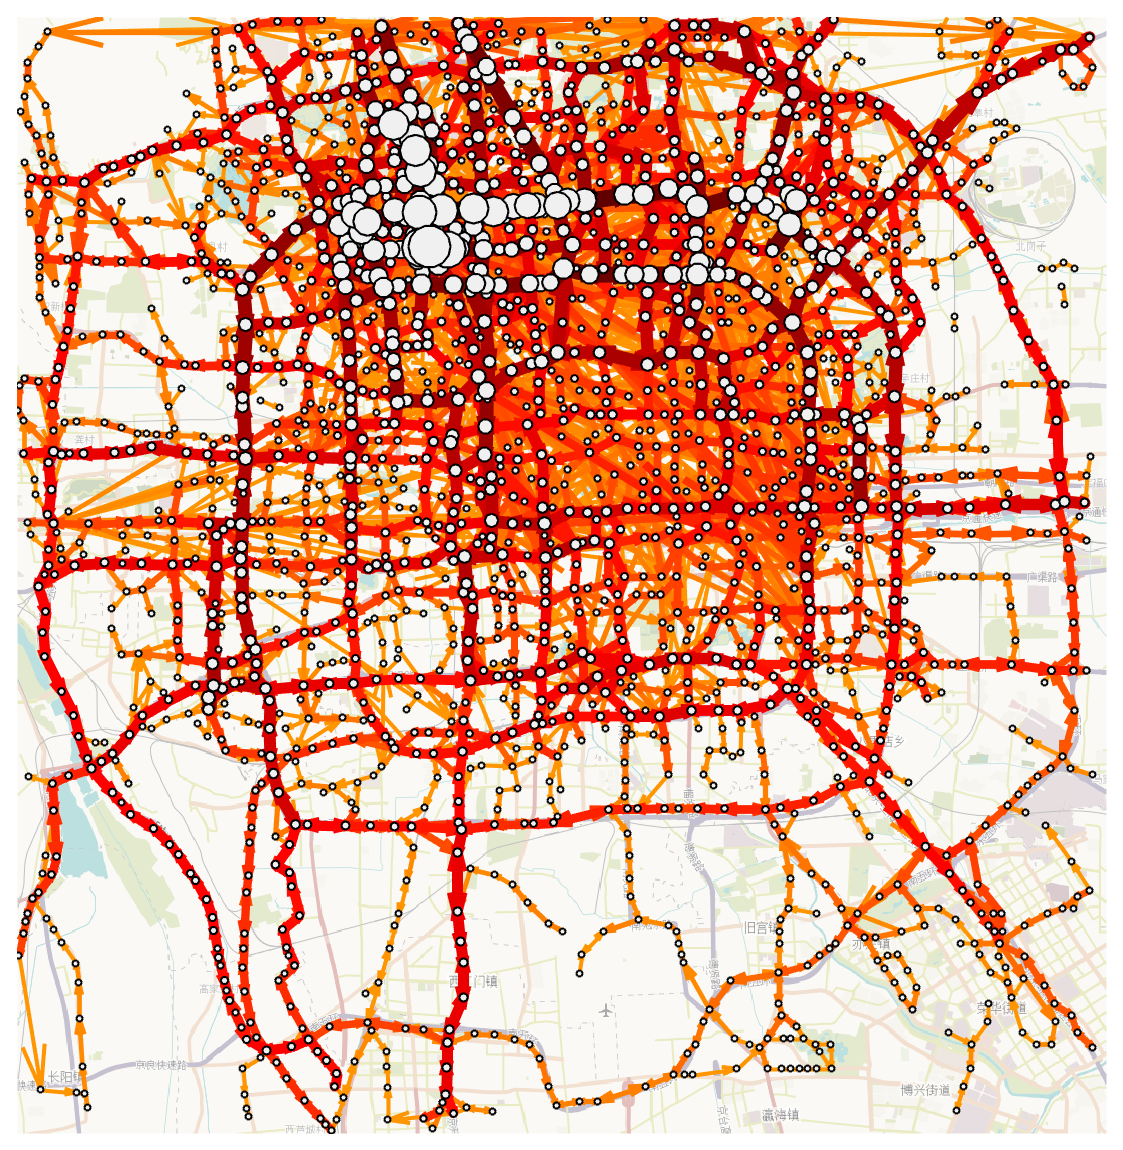
\includegraphics[width=32mm]{pics/geolife200m.eps}
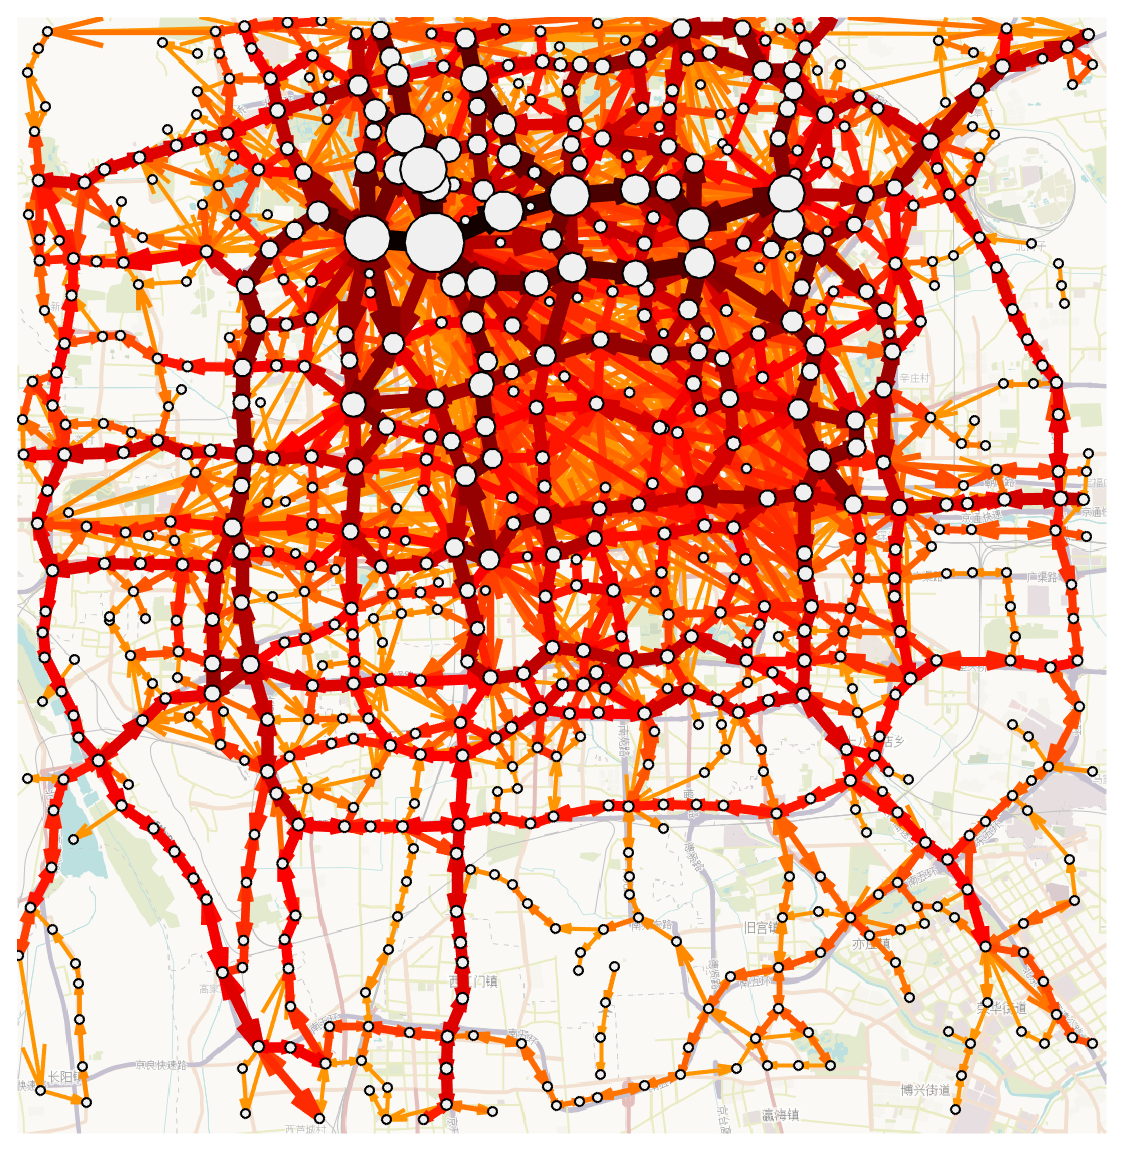
\includegraphics[width=32mm]{pics/geolife200_500m.eps}\\
(b) $\epsilon = 200$m  \hspace{5mm}(c) $\epsilon = 500$m\\
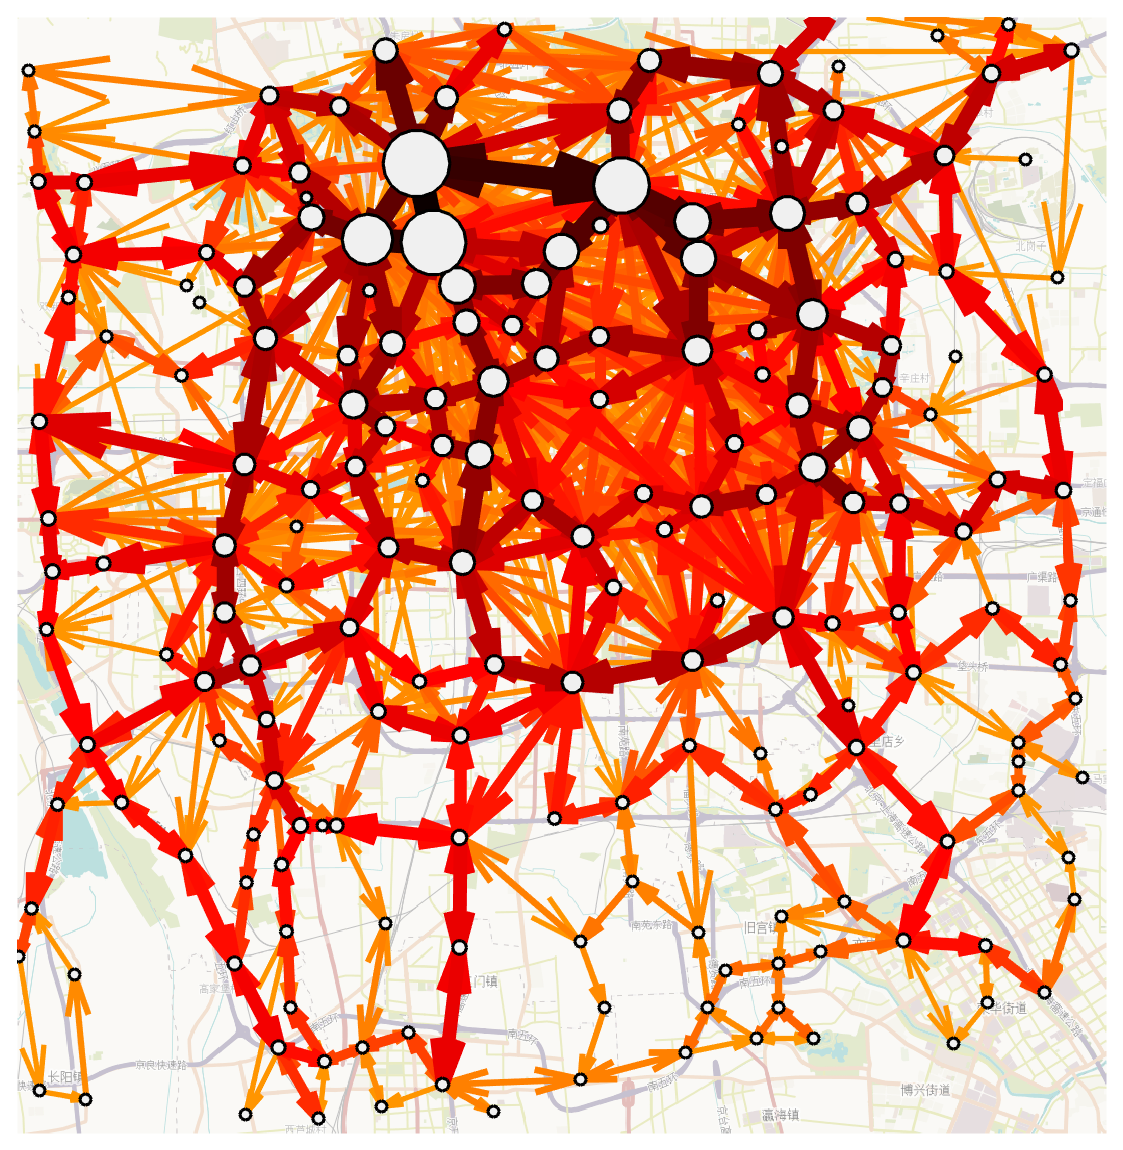
\includegraphics[width=32mm]{pics/geolife200_500_1000m.eps}
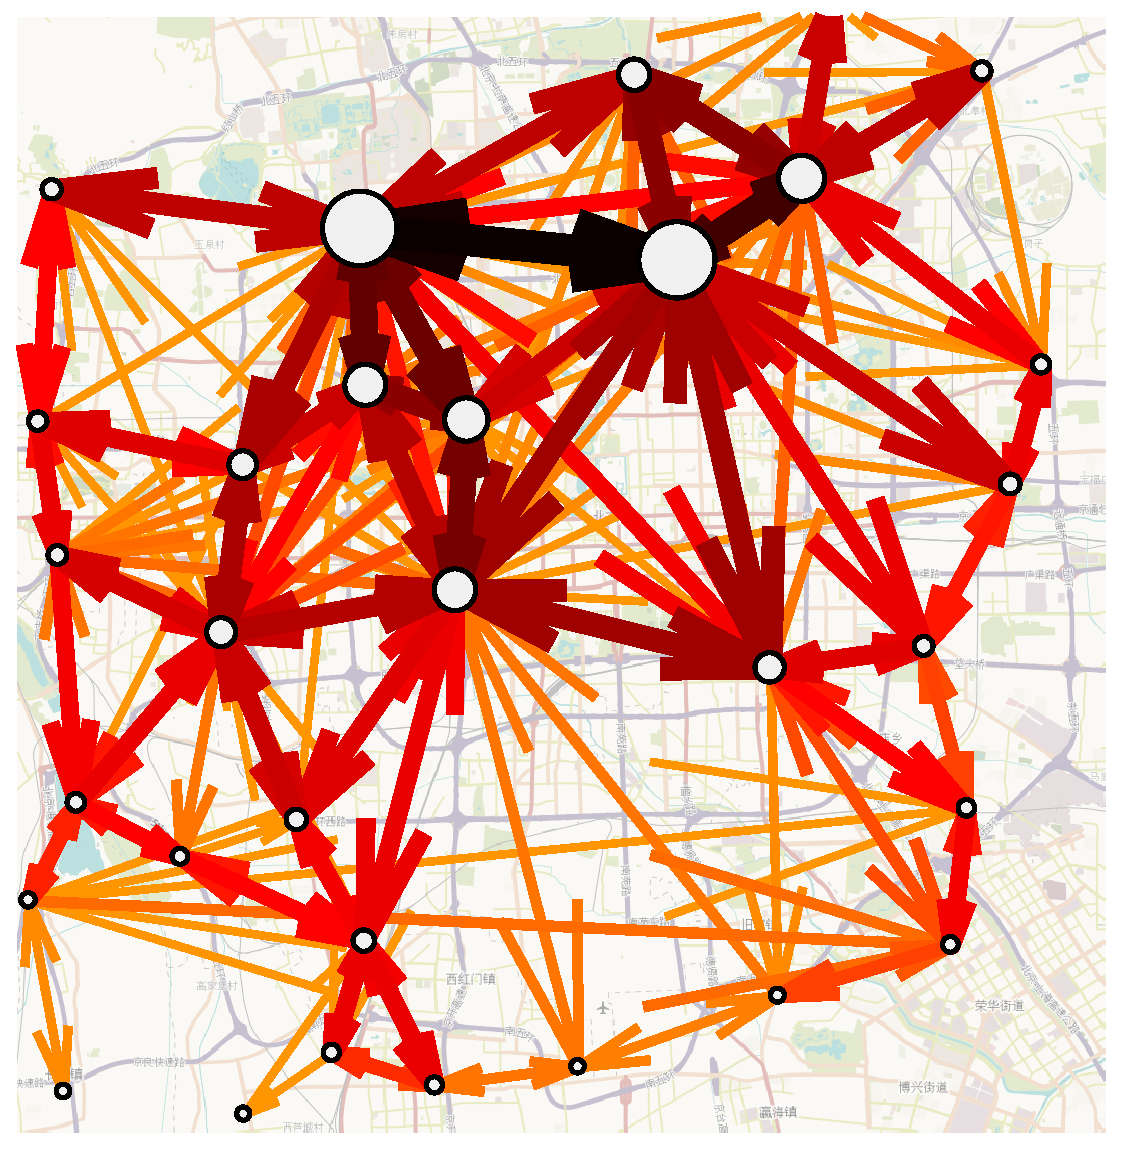
\includegraphics[width=32mm]{pics/geolife200_500_1000_3000m.eps}\\
\end{minipage}\\
(a) Geolife上的多层次ROI网络 & (d) $\epsilon = 1000$m  \hspace{5mm}(e) $\epsilon = 3000$m\\
\end{tabular}
\caption{在Geolife数据上的四层ROI网络。}
\label{fig:network}
\end{figure*}


\smallsection{对比算法}
由于在包含语义约束的数据中,轨迹压缩方法的性能不便于直接比较,我们为了证明\CascadeSync的有效性和高效性,使用五种主流的的轨迹压缩算法在特定实验上进行比较。
\emph{Douglas-Peucker} \citeup{douglas1973algorithms}: 是最有名的线简化算法,它使用贪婪策略检查第一个和最后一个点之间的所有点,直到最大空间偏差在误差范围$\zeta$内。算法复杂度为$\mathcal{O}(n^2)$。

\emph{Douglas-Peucker-SED} \citeup{meratnia2004spatiotemporal,potamias2006sampling}:是原算法的改版。其充分考虑了移动物体的时空特性,将原始的垂直距离度量换位了同步欧式距离(Synchronized Euclidean Distance, SED)。最坏的时间复杂度为$\mathcal{O}(n^2)$。

\emph{Dead Reckoning} \citeup{trajcevski2006line,muckell2011squish}:它是一种在线压缩模型。原理是通过当前位置和速度估算每个后继位置。通过计算估计位移和真实位置之间的偏差,如果偏差小于误差界限,则可以将点保持在压缩轨迹之外。时间复杂性是$\mathcal{O}(n)$。

\emph{Squish} \citeup{muckell2011squish,muckell2014compression}:使用了一个优先级队列,其中每个点的优先级被定义为若将该点的移除带来的误差。SQUISH通过从优先级队列中删除最低优先级的点来压缩每一条轨迹,直到达到目标压缩比或误差界限。Squish的时间复杂度为
$\mathcal{O}(\log n)$。

\emph{Traclus-MDL} \citeup{lee2007trajectory}:是一种固定压缩率的算法,其用最小描述长度(MDL)\citeup{grunwald2005advances} 来综合地描述模型的复杂度和表征能力,然后输出最平衡的一个压缩结果。其时间复杂度为$\mathcal{O}(n)$。

我们可以在给定误差范围的情况下与这些基线算法进行比较压缩比。此外,也可列出所有模型的压缩时间以比较效率。此外,我们还说明了\CascadeSync中语义ROI带来的影响。

\pic[!htb]{带语义ROI的Geolife上的多层次ROI网络}{width=125mm}{with}

\subsection{实验结果与分析}
% \subsection{基本性质的证明}
\smallsection{ROI网络可视化}
为了说明,我们首先可视化ROI网络。为了简洁起见,我们只能看到图\ref{fig:network}和图\ref{with}中的Geolife数据集上的多层ROI网络,它们是使用和不使用1000个固定交叉点的结果。 此外,从这些数据中,我们可以看到我们的模型在可视化方面是有效的,这可能为许多现实挖掘分析场景提供了基础。


\smallsection{表征误差分析}
与独立压缩每个轨迹的传统方法不同,我们基于同步的聚类模型 \CascadeSync将全局地压缩轨迹,并且代表性错误可以以很高地概率满足由$\zeta$的约束。我们将探索误差约束$\zeta$和交互范围$\epsilon$之间的关系。

在不失一般性的情况下,我们在Geolife数据集上进行此实验。24,876,978个 GPS点将被\Cascade表征为不同层次的ROI网络。我们将交互范围$\epsilon$从200米到2000米均匀地选择十次,大约是地图长度的$6/1000$到$60/1000$。通过增加模型中每层的交互范围,可以在不同级别的交互范围下计算所有点的平均代表性误差。其结果如图\ref{fig:relation}中的框图所示。框中的水平红线是中值,则蓝框的上边界是第三个四分位数,黑色虚线的上端表示最大值,超出最大值的红线被视为异常值。

没有预定义语义ROI的实验结果如图\ref{fig:relation}(a)所示,我们可以观察到误差最大值与交互范围$\epsilon$成正比,并且近似等于$\epsilon$。实际上,有$97.64\%$的点的表征误差小于$\epsilon$。换句话说,如果我们设置误差界为$\zeta=\epsilon$,没有语义ROI的\CascadeSync的结果将被$\zeta$以大于$0.9764$的概率约束住。

通过引入道路交叉点作为固定语义ROI,结果如图\ref{fig:relation}(b)。与之前不同,表征误差将先随着交互范围$\epsilon$的增加而增加,直到$\epsilon$达到$800$米,然后$\epsilon$继续增加而误差将保持不变。 在这个实验中,如果我们设置误差界为$ \zeta =\epsilon $,结果将以$ 0.9971 $的概率受$ \zeta $限制。

到目前为止,我们已经证明我们的方法\CascadeSync的误差将以非常高的概率被$ \zeta = \epsilon$所限制。此外,通过引入预定义的语义ROI,我们的模型还可以进一步减少表征误差。其原因很直观:更多的语义信息将会导致压缩结果中留有更多的语义ROI,但是,压缩比也会受到影响,我们将在下一个实验中展示。

\tabcolsep=3pt
\begin{figure}[!t]
\centering
% \footnotesize
% \vspace{-2mm}
\begin{tabular}{cc}
\includegraphics[width=70mm]{pics/relation_without2.pdf}&
\includegraphics[width=68mm]{pics/relation_with2.pdf}\\
(a) 没有语义ROIs & (b) 有语义ROI \\
\end{tabular}
\caption{代表性误差与相互作用范围之间的关系。框中的水平红线是中值,蓝框的上边界是第三个四分位数,黑色虚线的上端表示最大值,超出最大值的红线被认为是异常值。}
\label{fig:relation}
\end{figure}



\tabcolsep=0pt
\begin{figure*}[!htb]
\centering
% \footnotesize
\begin{tabular}{ccccc}
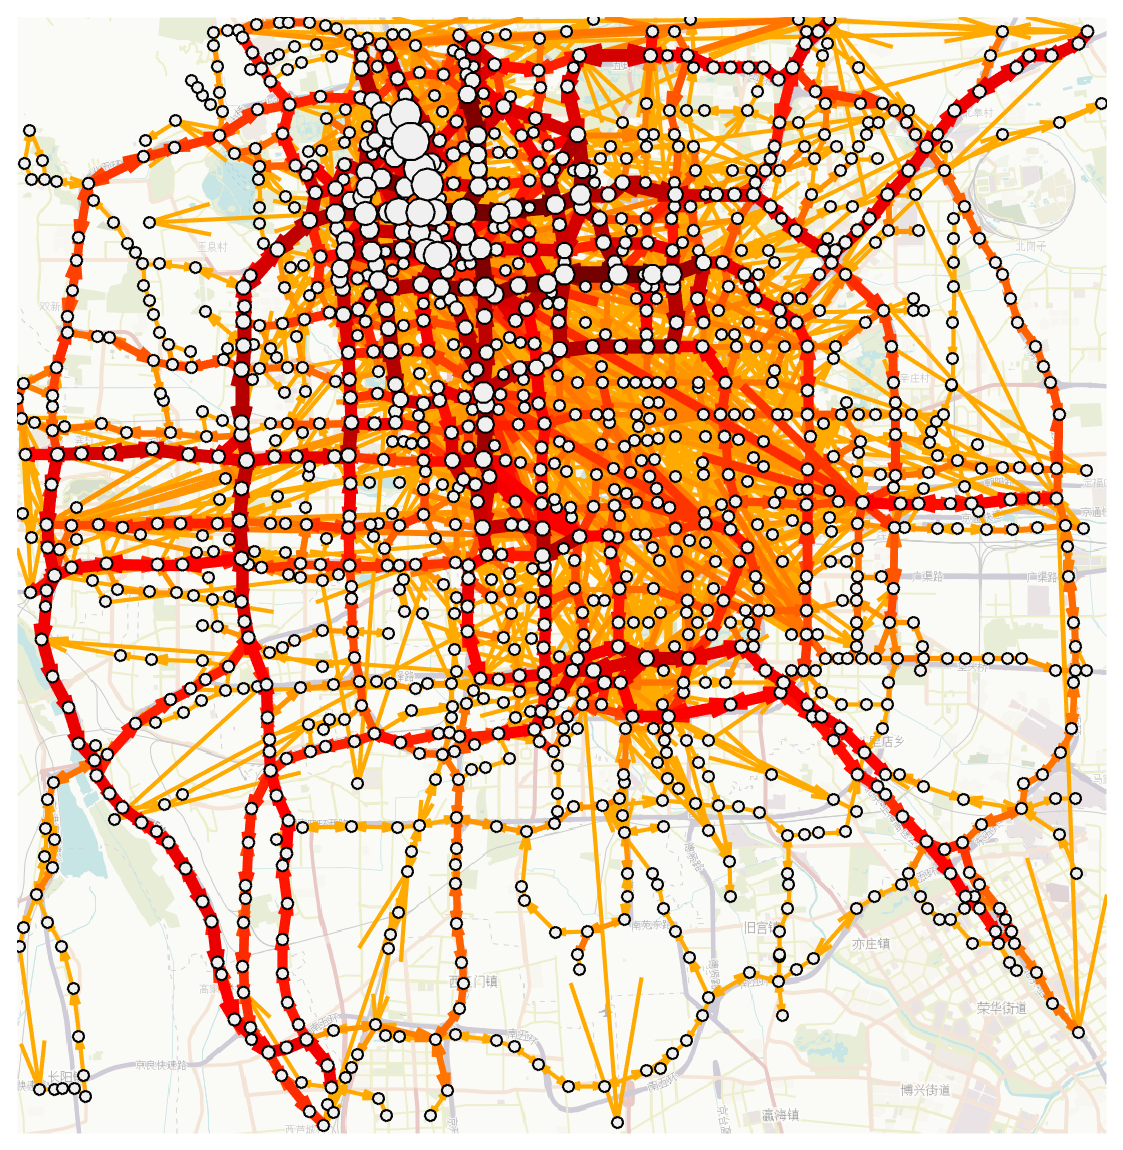
\includegraphics[width=35mm]{pics/Geolife200without.eps}&
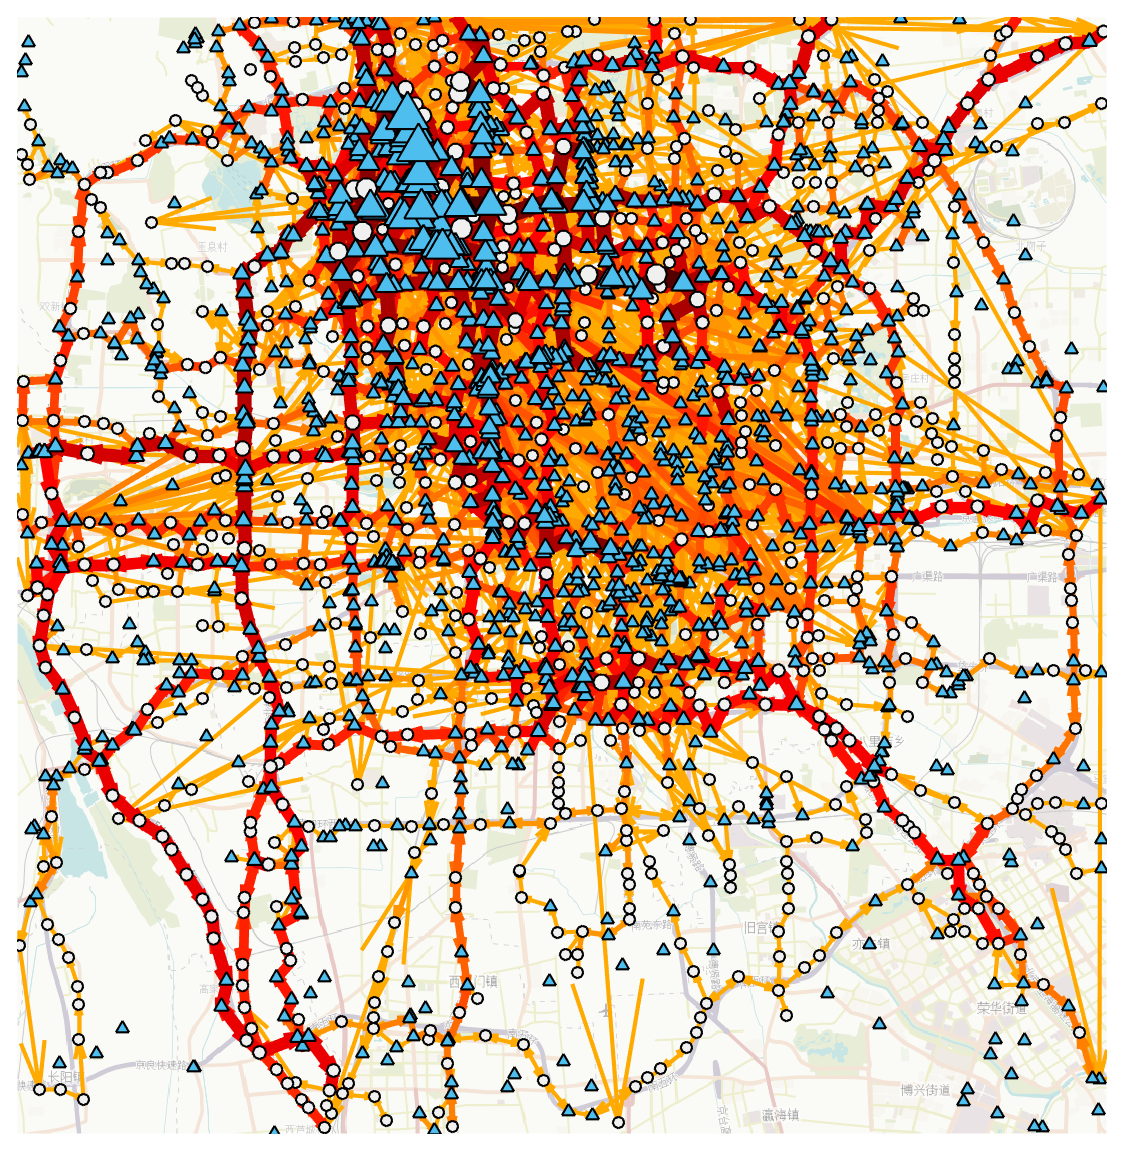
\includegraphics[width=35mm]{pics/Geolife200with.eps}&
~~&
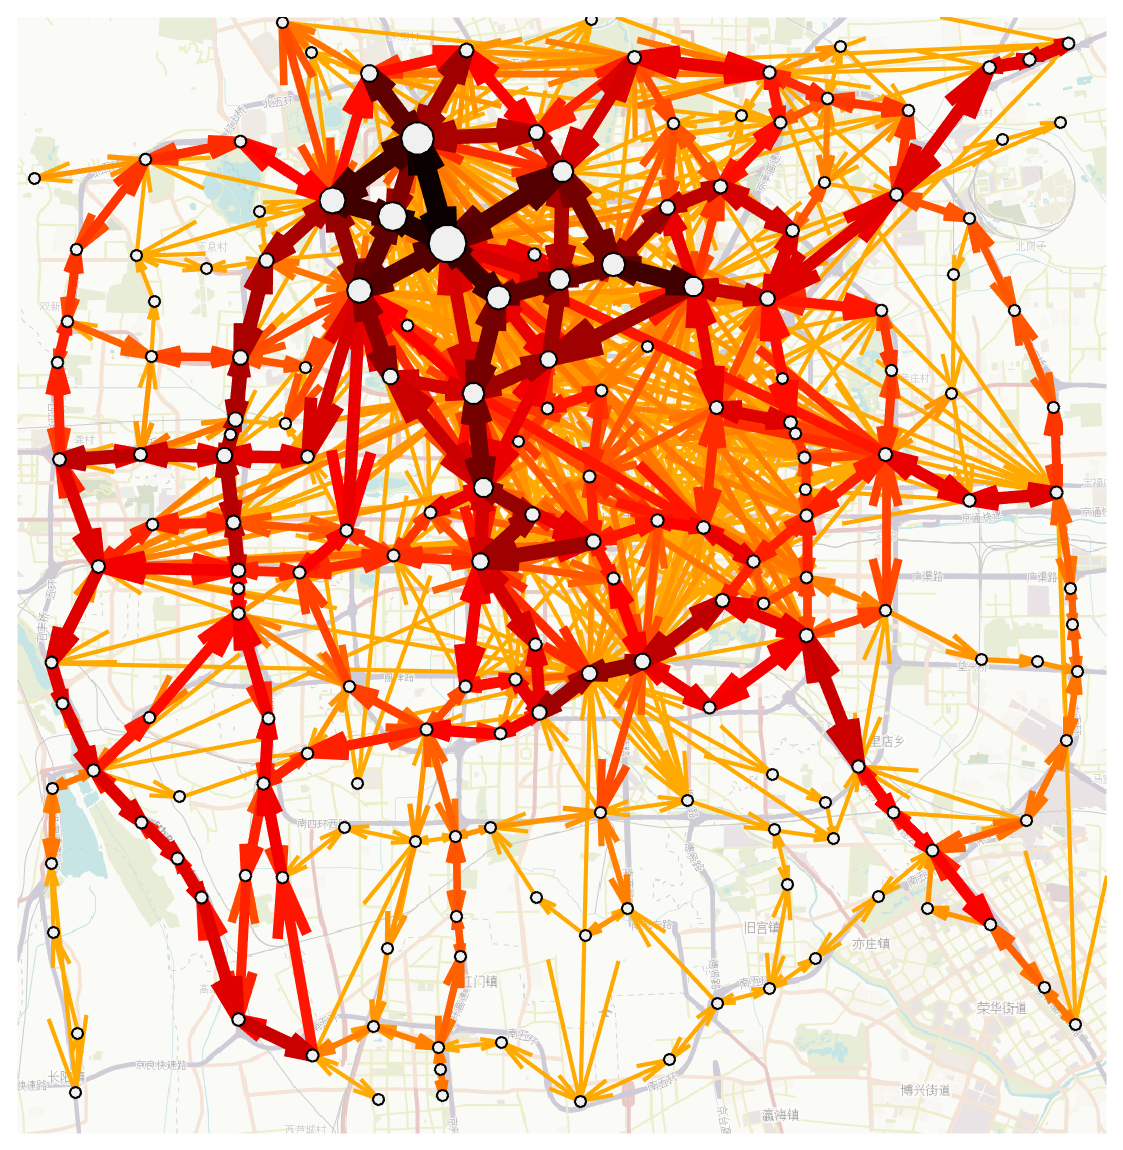
\includegraphics[width=35mm]{pics/Geolife1000without.eps}&
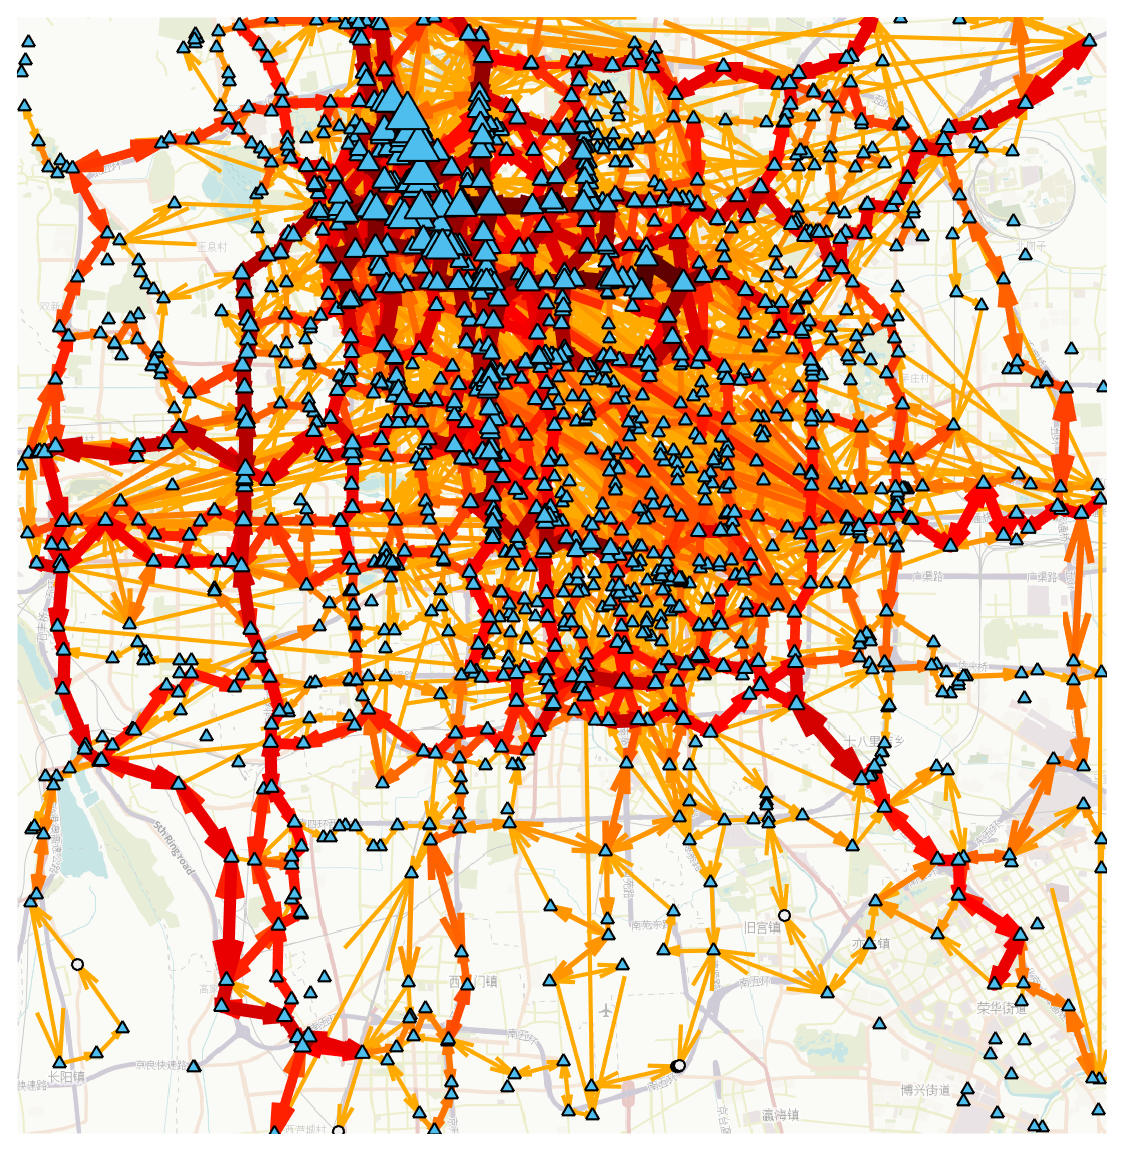
\includegraphics[width=35mm]{pics/Geolife1000with.eps}\\
% (a) Geolife: $\zeta = 200$m & (b) Geolife: $\zeta = 200$m & & (c) Geolife: $\zeta = 1000$m & (d) Geolife:$\zeta = 1000$m\\
\multicolumn{2}{c}{(a) Geolife: $\epsilon = 200$米} & & \multicolumn{2}{c}{(b) Geolife: $\epsilon = 1000$ (m)}\\
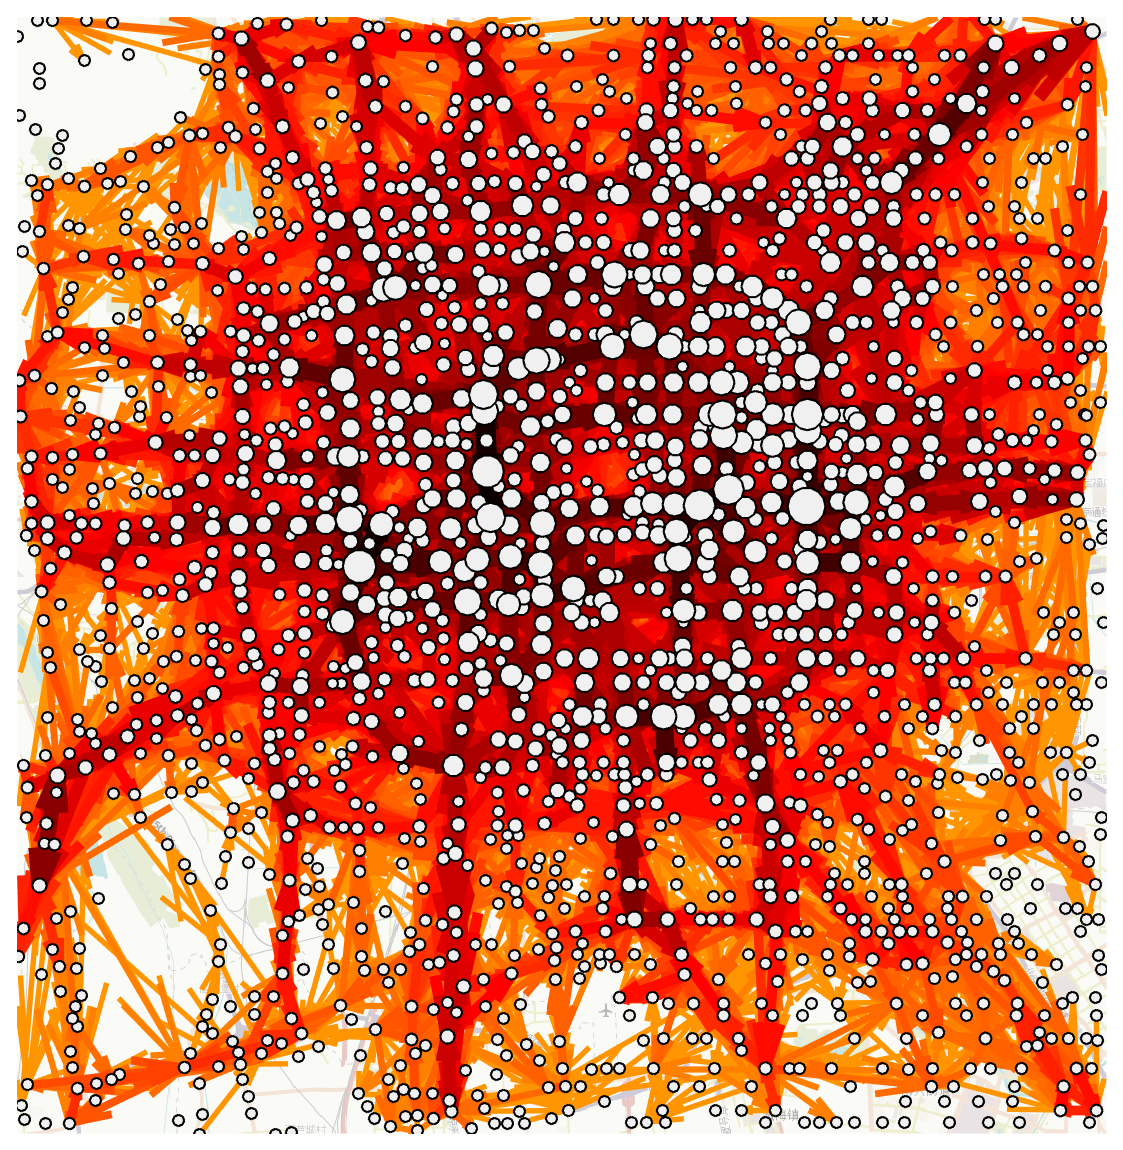
\includegraphics[width=35mm]{pics/tdrive200without.eps}&
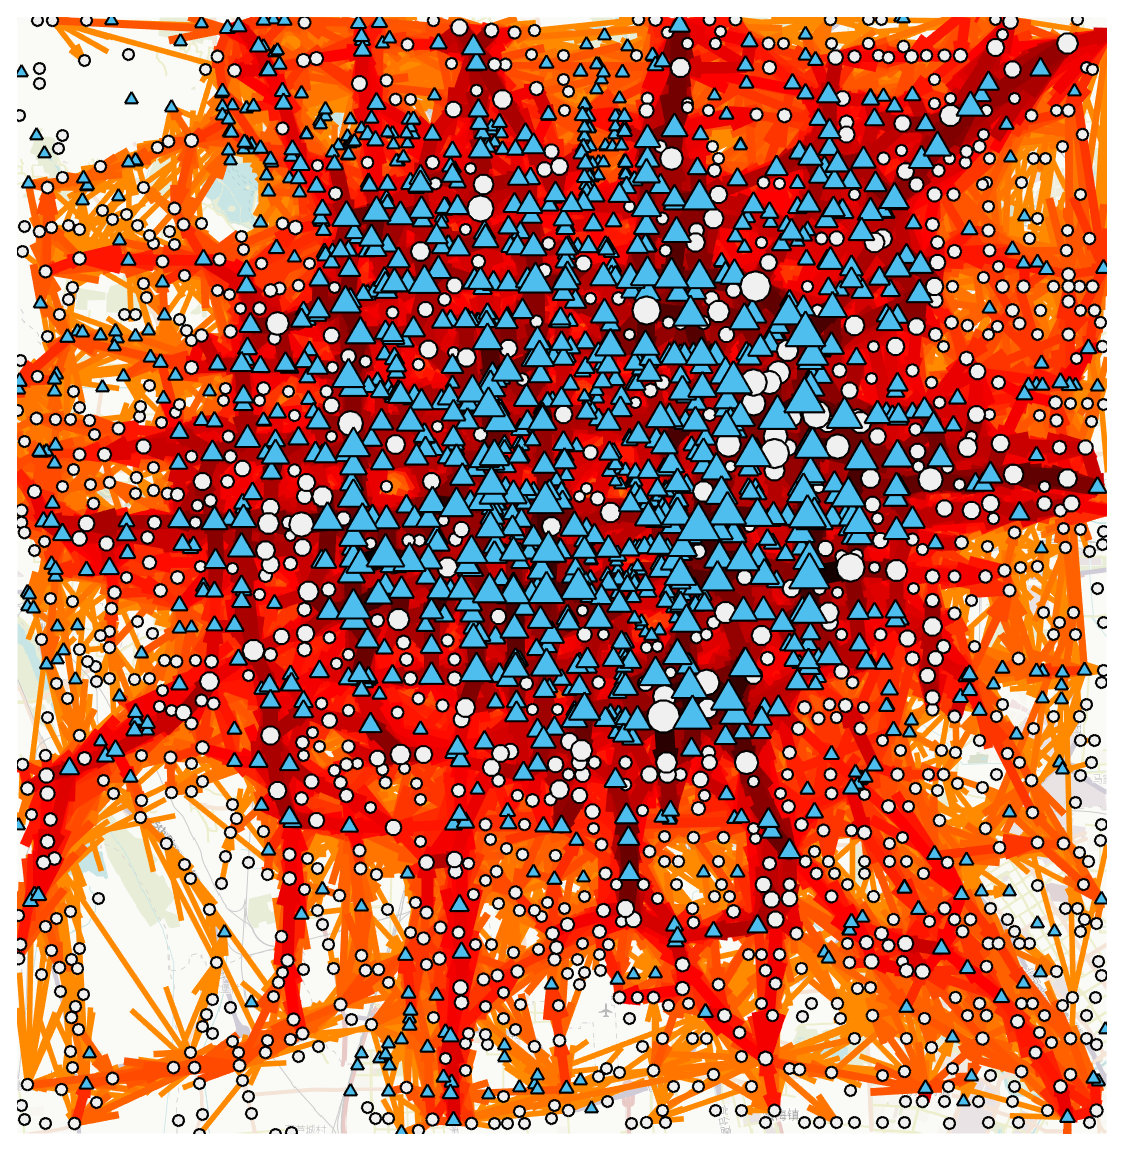
\includegraphics[width=35mm]{pics/tdrive200with.eps}&
~~&
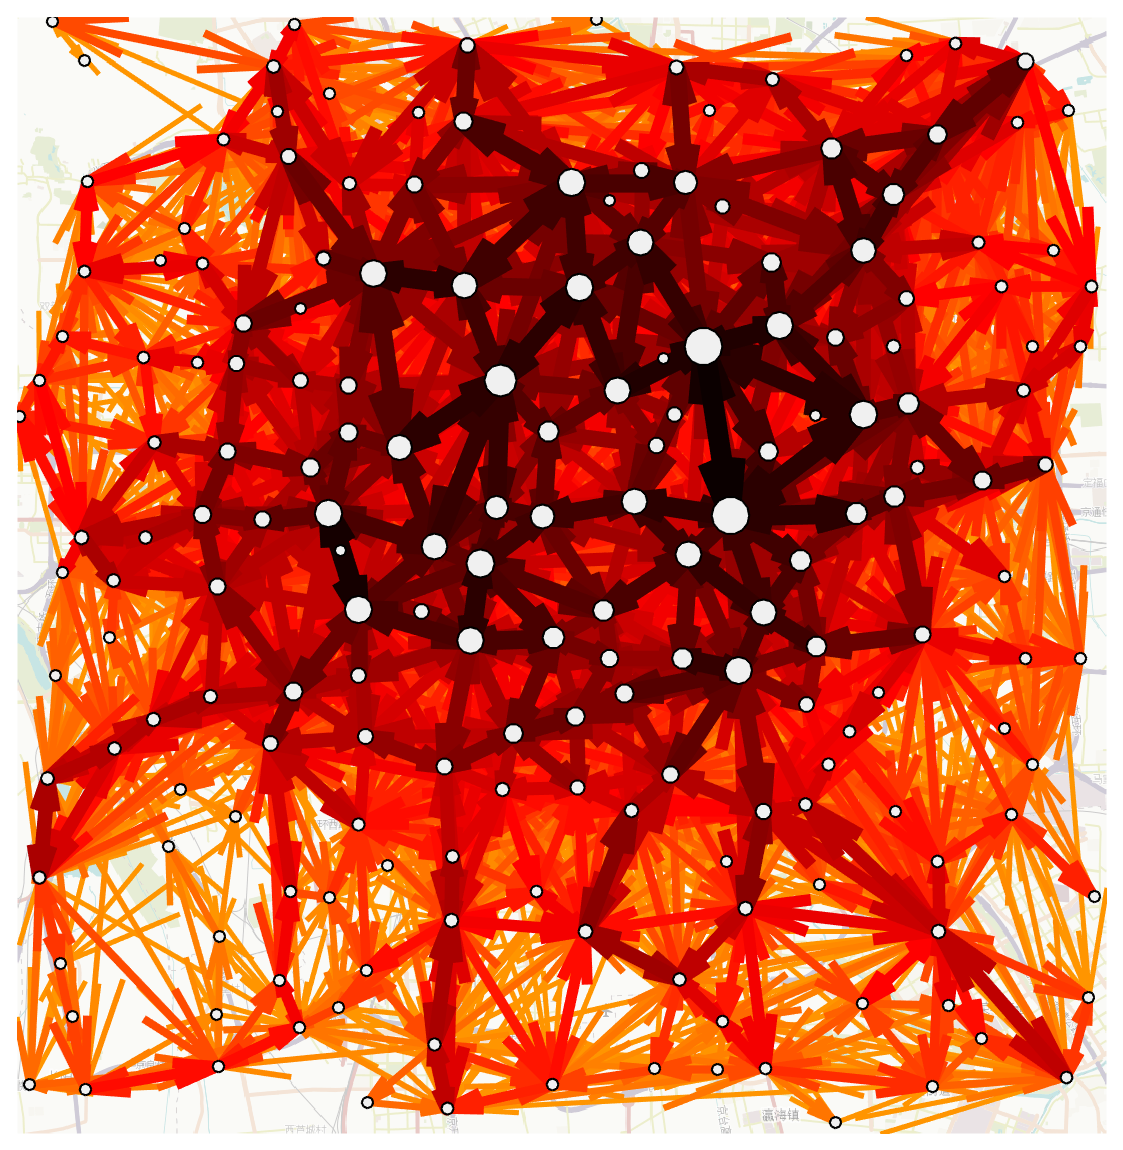
\includegraphics[width=35mm]{pics/tdrive1000without.eps}&
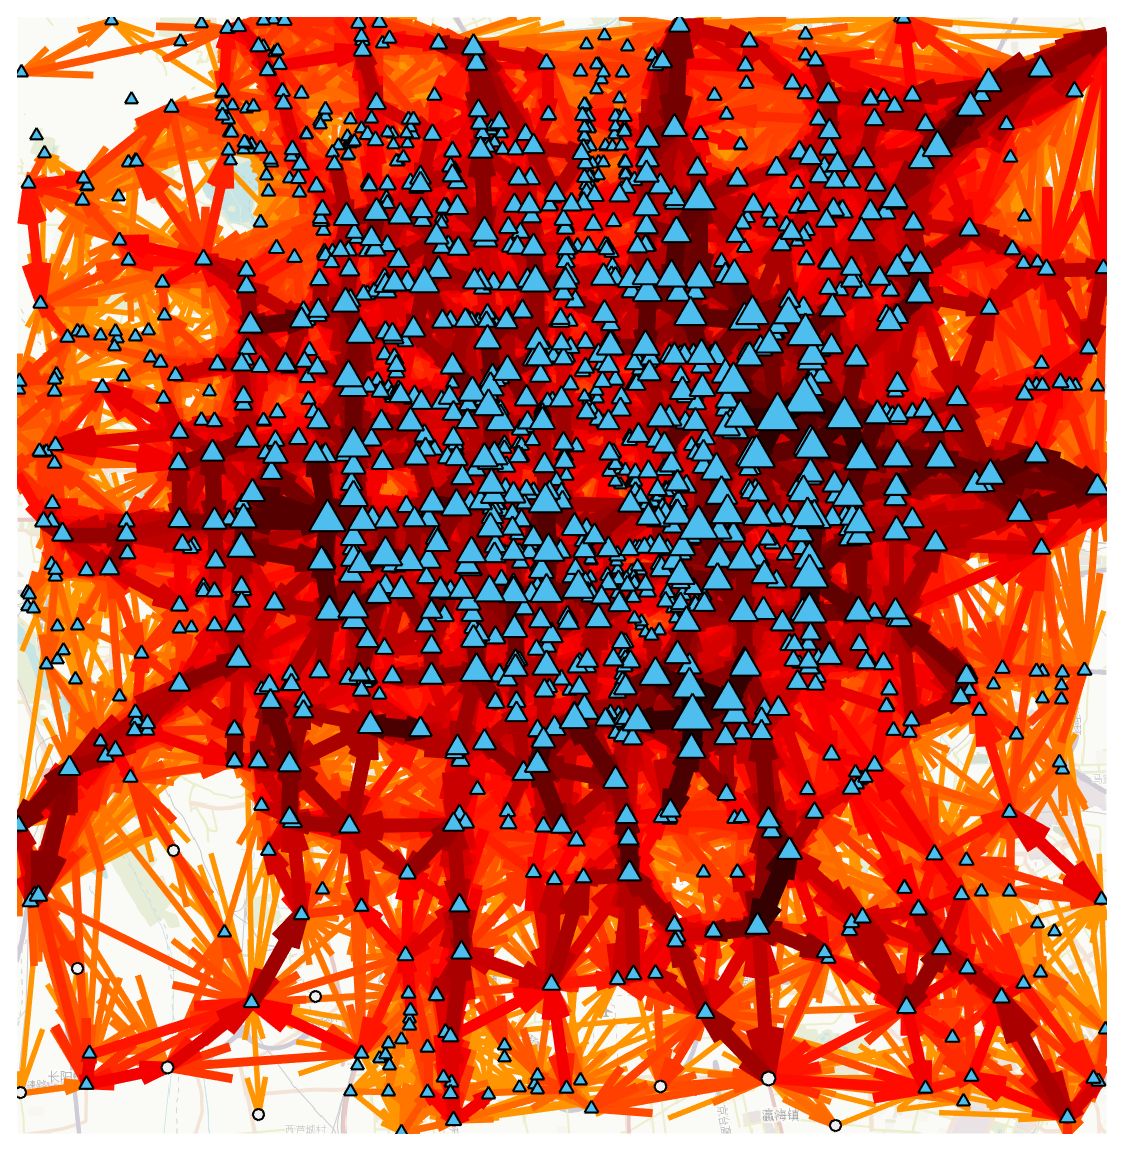
\includegraphics[width=35mm]{pics/tdrive1000with2.eps}\\
\multicolumn{2}{c}{(c) T-drive: $\epsilon = 200$ (m)} & & \multicolumn{2}{c}{(d) T-drive: $\epsilon = 1000$ (m)}\\
\multicolumn{5}{c}{
\begin{minipage}[b]{138mm}\centering

\begin{minipage}[b]{35mm}\centering
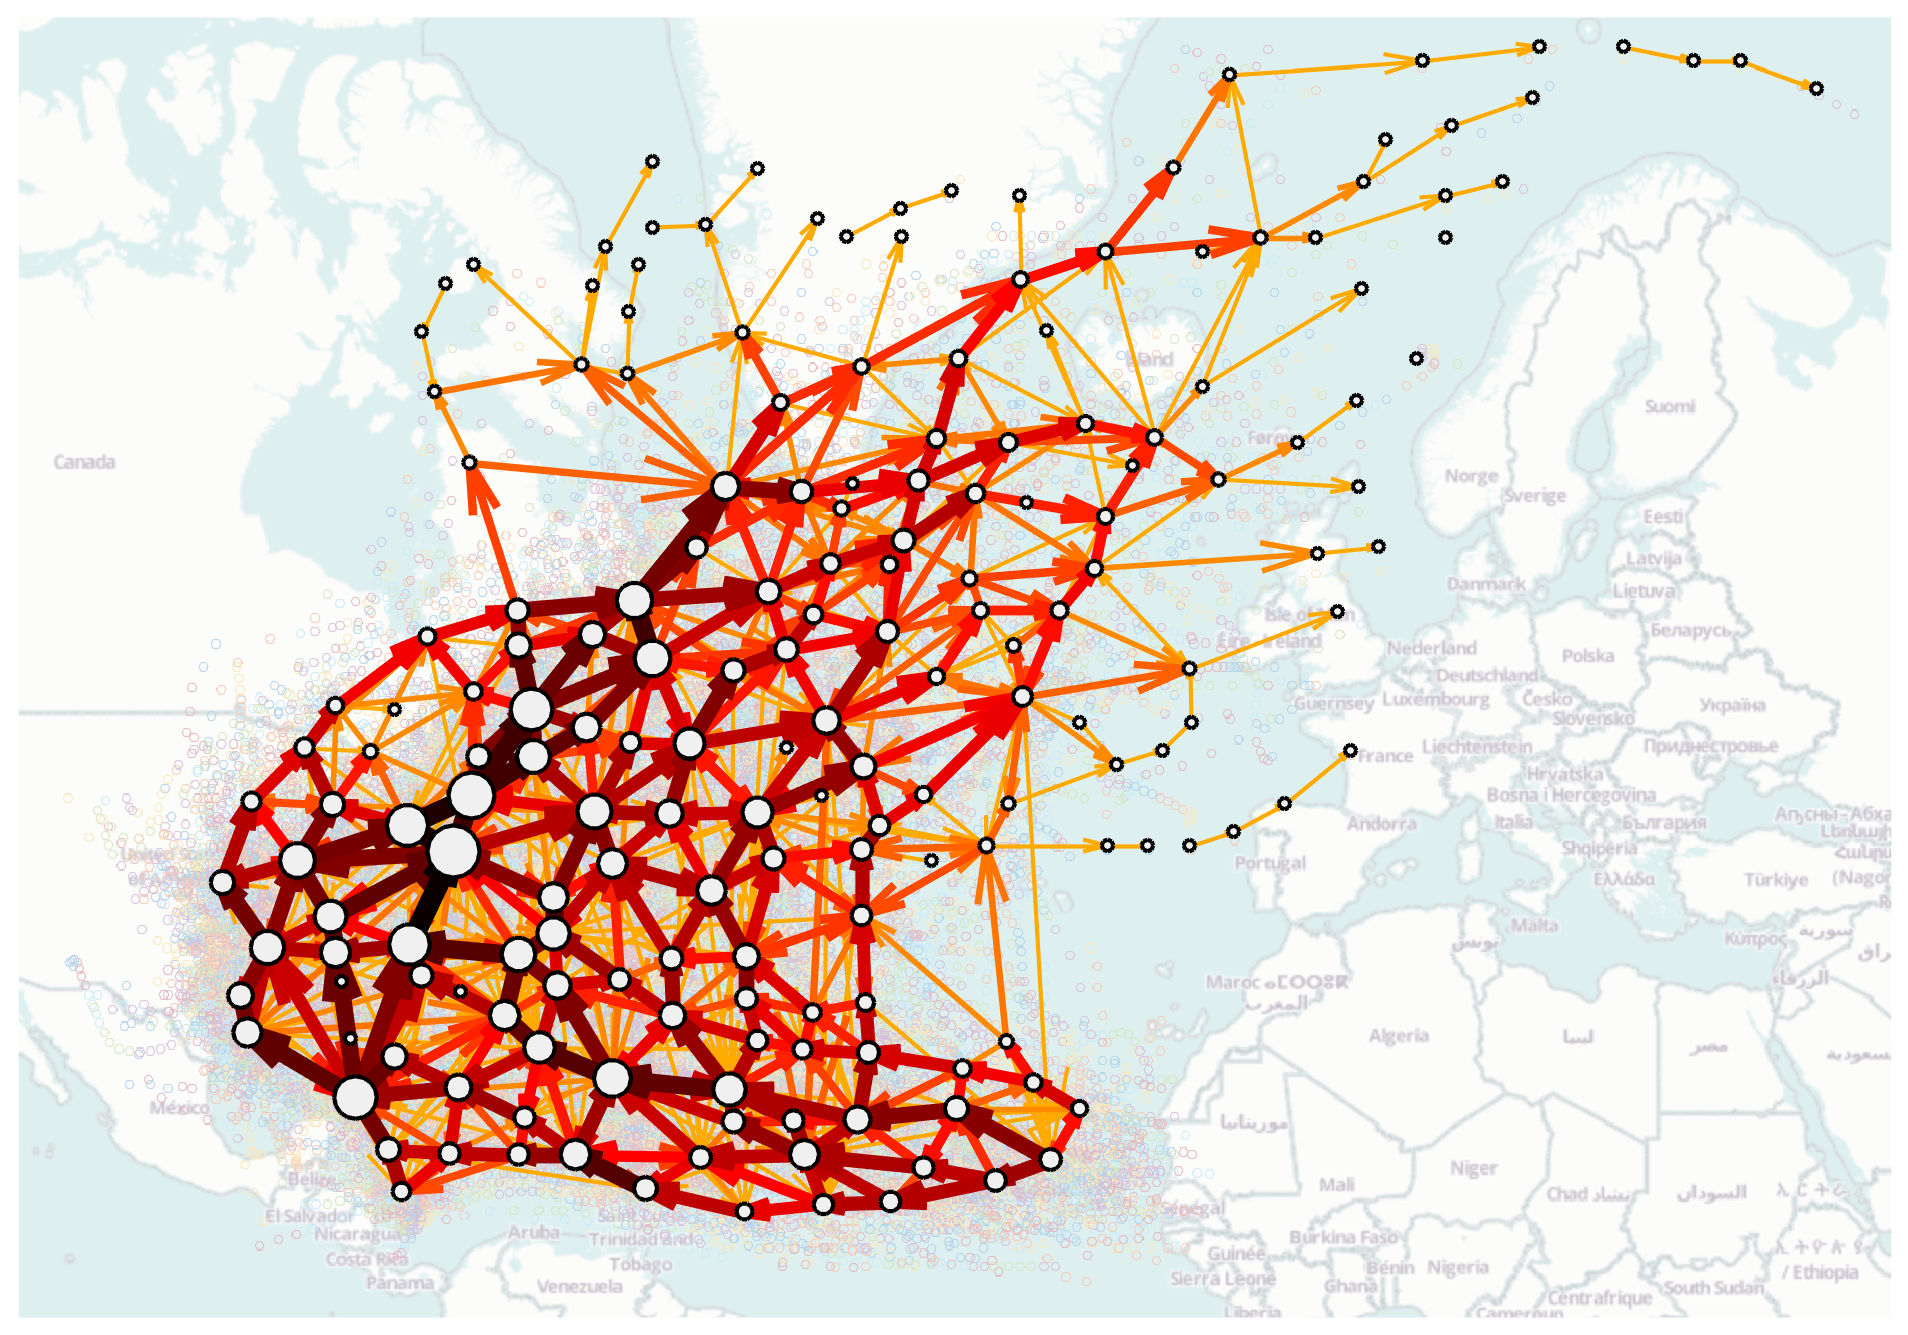
\includegraphics[width=34mm]{pics/Hurricane_2.eps}\\
(e)  $\epsilon = 180$ (km) \\
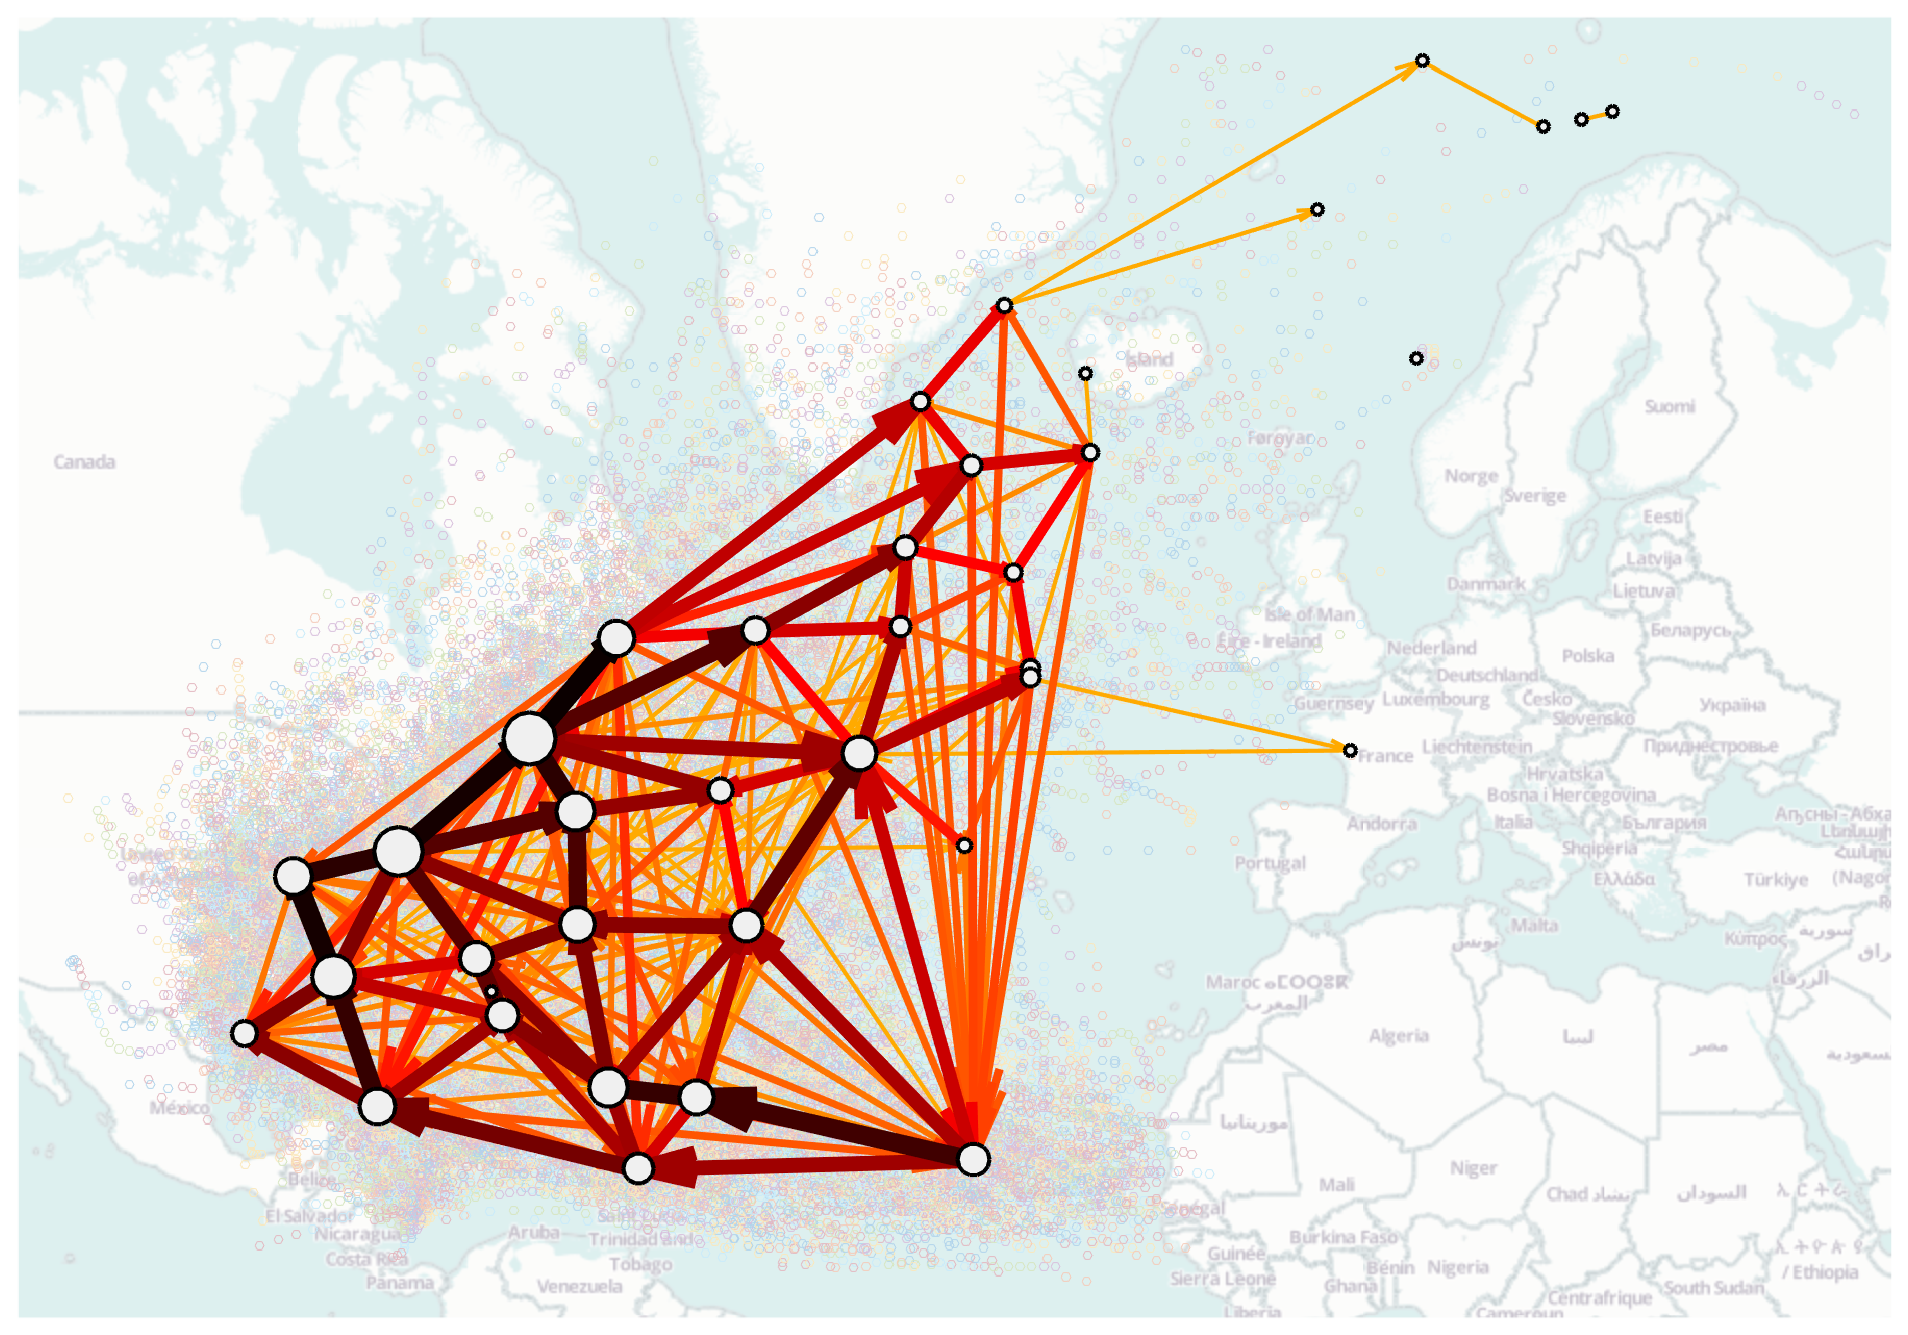
\includegraphics[width=34mm]{pics/Hurricane_4.eps}
(f)  $\epsilon = 540$ (km)
\end{minipage}
\begin{minipage}[b]{101mm}\centering
\includegraphics[width=33mm]{pics/Migration_2-eps-converted-to.pdf}
\includegraphics[width=33mm]{pics/Migration_5-eps-converted-to.pdf}
\includegraphics[width=33mm]{pics/Migration_8-eps-converted-to.pdf}\\
(g) $\epsilon = 10$ (km)  ~~~~(h) $\epsilon = 30$ (km) ~~~~ (i) $\epsilon = 50$ (km) \\
\end{minipage}
\end{minipage}
}\\
\end{tabular}
\caption{ROI网络在在不同的数据集上不同误差界的结果。在每一个子图中,左手边的ROI网络是没有固定语义ROI的约束的结果,右边的结果加入了1000个随机选择的十字路口。}
\label{fig:illustration}
\end{figure*}

\smallsection{压缩率分析}
在本节中,我们进行压缩率的比较,以显示\CascadeSync的出色表征能力。注意不同的算法应该使用相同的误差界$\zeta $,以便我们可以直接比较性能。我们在\CascadeSync中设置$\zeta = \epsilon $,这是依据了上面结果中结果将会以以高概率(大于$97\%$)满足这个条件。

\CascadeSync将在Geolife和T-Drive数据上使用两次,其中不同之处在于是否使用了预定义的交叉点(即语义信息)。通过在合理范围内改变误差约束$ \zeta $的值,我们将四个数据集的压缩比呈现在结果\ref{fig:ratio}中。而一些结果ROI网络将在\ref{fig:illustration}中被可视化。

结果中,四个数据集上压缩比的比例是不同的。例如,Geolife和T-drive都是北京的轨迹。然而,Geolife的采样率是T-drive的数百倍。因此,Geolife中包含更多冗余,从而产生非常高的压缩比。图\ref{fig:illustration}(a)-(d)中的ROI网络也显示着这一差异。T-drive的ROI网络比Geolife更复杂,这表明轨道上存在许多空缺区域。

尽管如此,四个模型的压缩比在每个数据集中是可以横向比较的。Douglas-Peucker优于其他模型,我们的\CascadeSync在没有语义ROI中随着误差界的增加而倾向于超越其他模型。重要的是要注意Traclu-MDL呈现扁平的结果,这是因为模型不将误差界作为参数,因此无法控制压缩比。同时,\CascadeSync在具有语义信息下并不擅长控制压缩率,这种现象也可以通过图\ref{fig:illustration}ROI网络揭示出来。通过增加误差界限$\zeta$,正常ROI开始减少,道路交叉点逐渐成为地图上起主导地位的ROI。

实验表明,\CascadeSync具有出色的压缩比和表征能力。现在我们通过比较运行时与其他算法来展示\CascadeSync最显着的特性。我们报告了六种算法对四种真实数据的运行时间。每个算法在每个数据集上运行十次,平均运行时间统计结果如表\ref{tab:times}中所列。请注意,表\ref{tab:times}和图\ref{fig:ratio}中的压缩比是在统一的实验中同时测量的。\CascadeSync比其他五种方法快数千倍。这是因为传统模型逐个压缩轨迹,因此运行时间与数据集中的点成比例。我们的模型在全局范围内进行,因此点数将呈指数级减少,这大大加速压缩过程。




\tabcolsep=0pt
\begin{figure}[!htb]
\centering
% \footnotesize
\begin{tabular}{cc}
\includegraphics[width=60mm]{pics/geolife.pdf}&
\includegraphics[width=60mm]{pics/tdrive.pdf}\\
(a) Geolife & (b) T-drive \\
\includegraphics[width=60mm]{pics/hurricane.pdf}&
\includegraphics[width=60mm]{pics/Migration.pdf}\\
(c) Hurricane & (d) Migration\\
\end{tabular}
\caption{在四个数据集上压缩率—误差界变化曲线图。}
\label{fig:ratio}
\end{figure}


\tabcolsep=2pt
\begin{table}[!htb]\renewcommand{\arraystretch}{1.3}
\vspace{1mm}
\caption{在四个数据集上的速率对比,单位:秒。}
\center
\small
\begin{tabular}{lcccccc}
\hlinew{1pt} \textbf{}& \textbf{~~DP~~}& \textbf{~~DP-SED~~} & \textbf{~~DR~~} & \textbf{Squish} & \textbf{Traclus-MDL} & \textbf{CascadeSync}\\ 
\hlinew{1pt}
\textbf{Geolife}  & 6100.42 & 36621.08 & 14525.53 & 14712.10 & 6357.91 & \textbf{15.38}\\
\textbf{Tdrive}   & 2288.57 & 35422.91 & 5101.41 & 5289.05 & 2344.51 & \textbf{7.51}\\
\textbf{Hurricane}& 16.46 & 49.80 & 30.98 & 33.54 & 13.78 & \textbf{0.42}\\
\textbf{Migration}& 1.79 & 12.09 & 4.40 & 4.44 & 2.28 & \textbf{0.10} \\
\hlinew{1pt}
\end{tabular}
\label{tab:times}
\end{table}


\tabcolsep=5pt
\begin{table*}[!htb]\renewcommand{\arraystretch}{1.3}
\caption{Geolife数据集上的时空查询结果。}
% \vspace{1mm}
\center
\small
\begin{tabular}{c|c|c|c|c|c}
\hlinew{1pt}
\multicolumn{3}{c|}{\textbf{轨迹时空查询}} & \multicolumn{3}{c}{\textbf{轨迹条数}} \\
\hlinew{1pt}
编号 & 地点 & 时间范围 & $\epsilon = 500m$ & $\epsilon = 1000m$ & $\epsilon = 3000m$\\
\hlinew{.85pt}
\multirow{2}{*}{1}& 北京大学 & \multirow{2}{*}{2008-11-28,2009-01-07} &\multirow{2}{*}{3} & \multirow{2}{*}{8} & \multirow{2}{*}{51}\\
& 金融街 & & & & \\
\hline
\multirow{2}{*}{2}& 王府井 & \multirow{2}{*}{2009-02-14,2009-03-20} &\multirow{2}{*}{4} & \multirow{2}{*}{18} & \multirow{2}{*}{44}\\
& 北京西站 & & & & \\
\hline
\multirow{3}{*}{3}& 天安门广场 & \multirow{3}{*}{2009-01-27,2009-02-25} &\multirow{3}{*}{0} & \multirow{3}{*}{2} & \multirow{3}{*}{9}\\
& 北京站, & & & & \\
& 国家体育馆 & & & & \\
\hline
\multirow{3}{*}{4}& 中关村 & \multirow{3}{*}{2008-06-18,2008-06-22} &\multirow{3}{*}{1} & \multirow{3}{*}{2} & \multirow{3}{*}{12}\\
& 光熙门, & & & & \\
& 建国门 & & & & \\
\hline
\multirow{3}{*}{5}& 天坛公园 & \multirow{3}{*}{2008-04-02,2009-11-23} &\multirow{3}{*}{15} & \multirow{3}{*}{139} & \multirow{3}{*}{578}\\
& 故宫, & & & & \\
& 北海公园 & & & & \\
\hlinew{1pt}
\end{tabular}
\label{tab:retrieval}
\end{table*}

\tabcolsep=1pt
\begin{figure*}[!t]
\centering
% \footnotesize
\begin{tabular}{ccc}
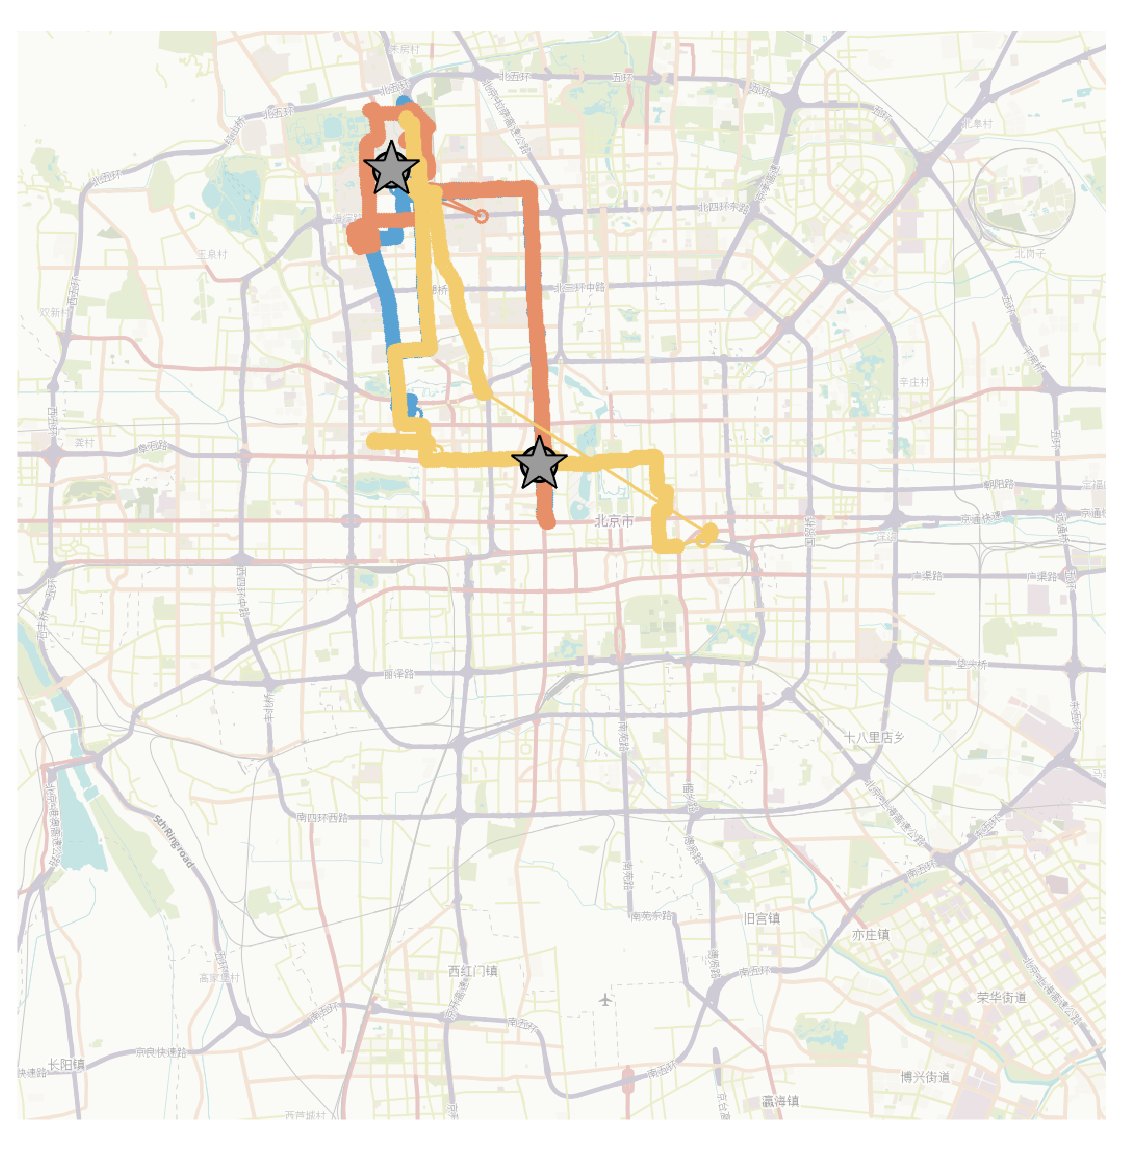
\includegraphics[width=48mm]{pics/q500.eps}&
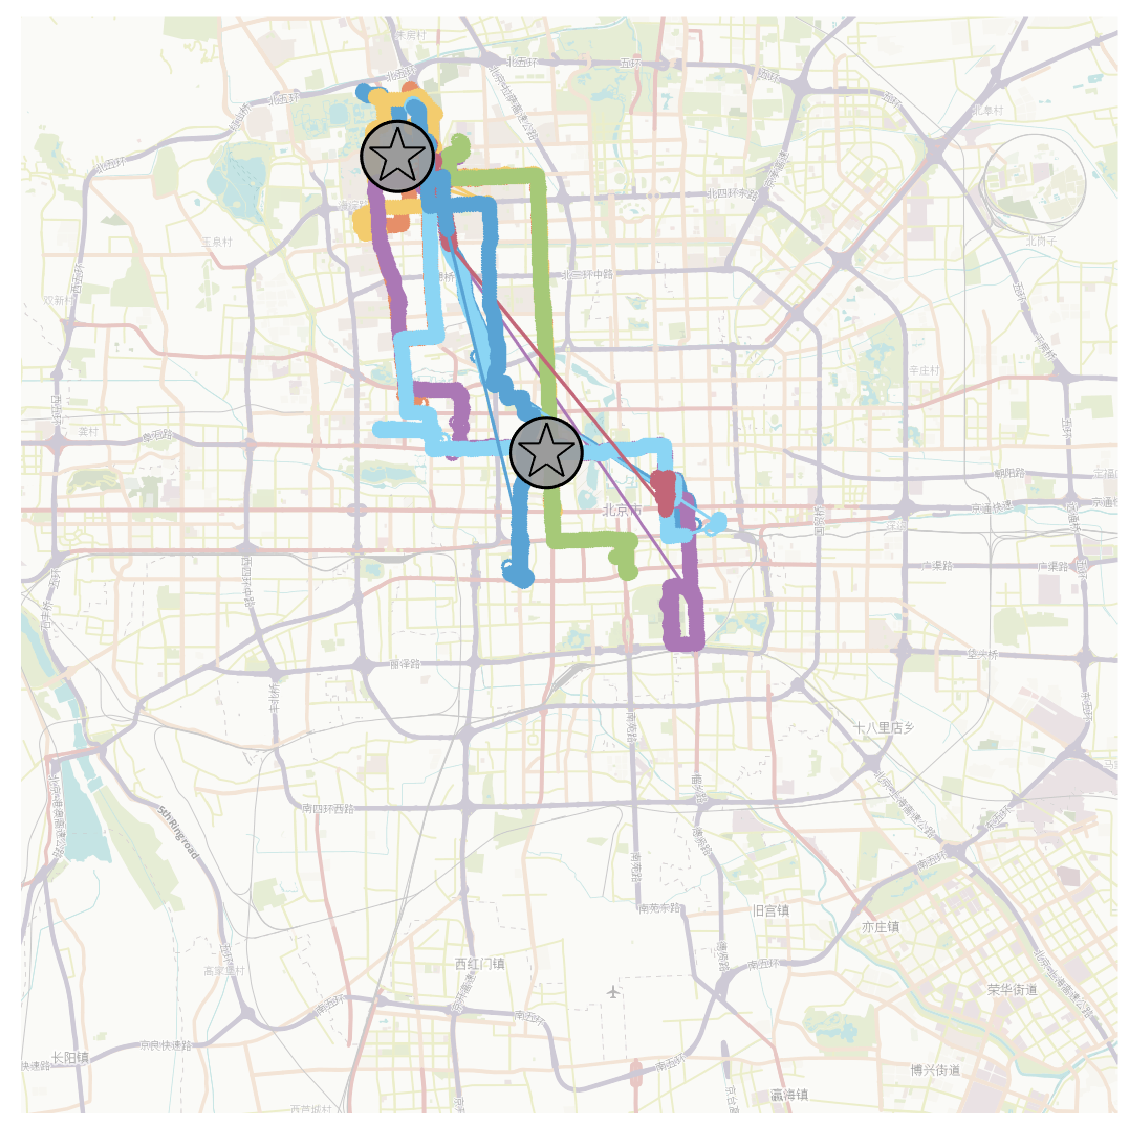
\includegraphics[width=48mm]{pics/q1000.eps}&
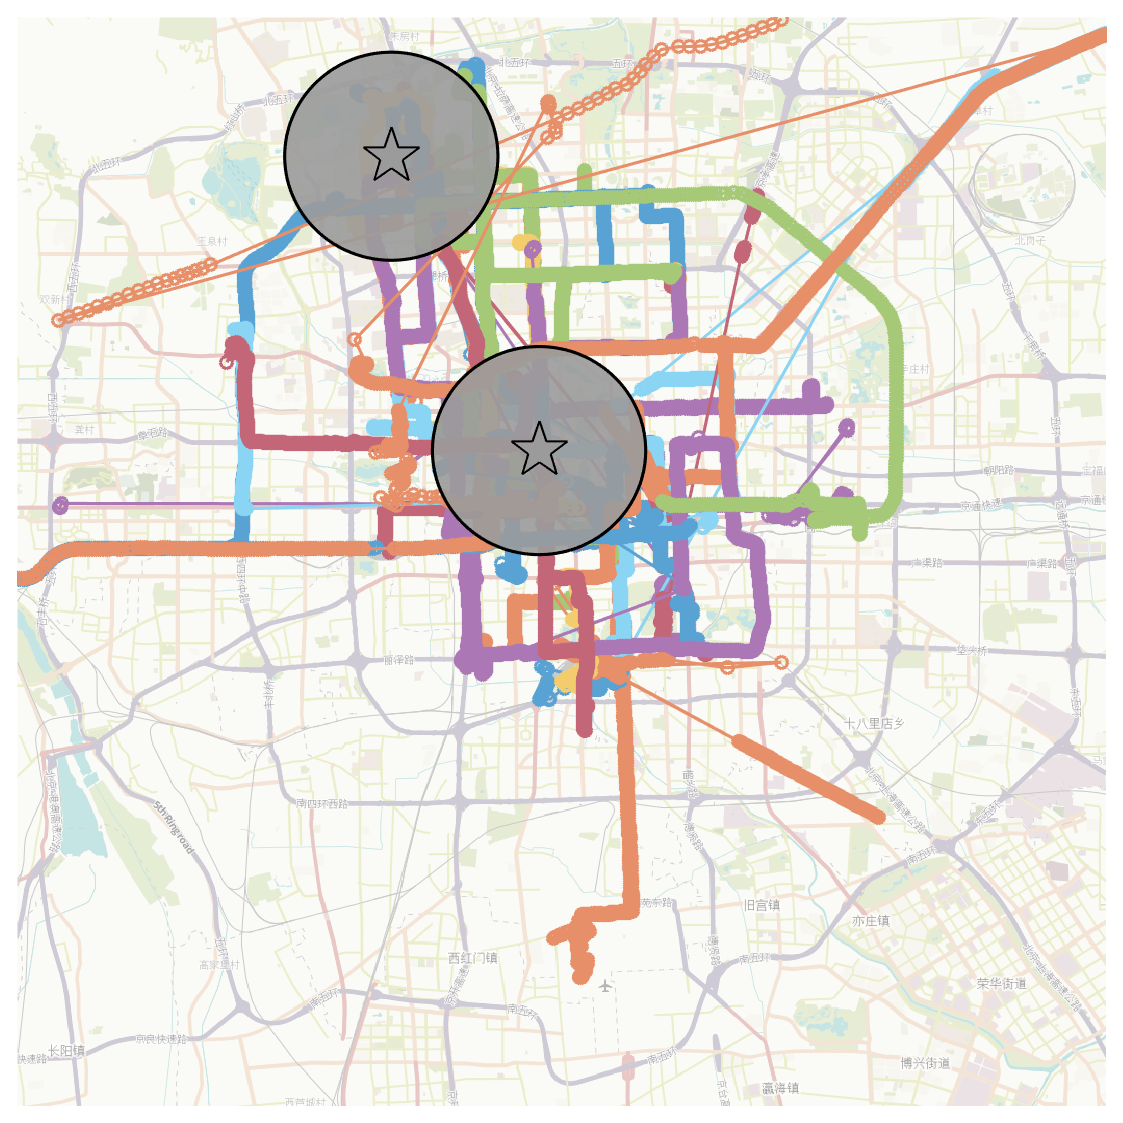
\includegraphics[width=48mm]{pics/q3000.eps}\\
(a) $\epsilon = 500m$, \#Traj.=3 & (b) $\epsilon = 1000m$, \#Traj.=8 & (c) $\epsilon = 3000m$, \#Traj.=51  \\
\end{tabular}
\caption{不同搜索范围的轨迹时空轨迹检索结果。这里检索了两个地点北京大学和金融街。 时间范围从2008-11-28到2009-01-07。 圆的半径表示交互范围范围$\epsilon$
}
\label{fig:queryResult}
\vspace{2mm}
\end{figure*}

\smallsection{轨迹的时空查询}
ROI网络是轨迹数据的一种紧凑表示,在ROI网络上可以总结全局信息和特殊语义信息,这可以促进后续应用。在本节中,我们以时空检索任务为例。给定城市中的一组地标或区域以及时段,我们检索在相应时段内通过所有这些地段或者区域的轨迹。由于我们的多层次ROI网络记录了通过轨迹的访问时间,因此可以通过在已有ROI网络上应用算法\ref{alg:query}来轻松检索轨迹。

为简单起见,我们只说明Geolife上的查询结果,并执行五个查询。由于在 Geolife数据上,大多数轨迹都位于微软亚洲研究院(MSRA)和一些大学的校园附近,因此覆盖整个北京城市的轨迹很少。这里我们只考虑三个范围(500米,1000米和3000米)。如在图\ref{fig:queryResult}中给出2008-11-28至2009-01-07的第一个检索结果。当$\epsilon$设置为500米时,穿过北京大学和金融街的共同轨迹只有3条,而随着交互范围$ \epsilon $的增加,结果数量自然会上升。

实验表明,在给定的特定点和相应的时间范围内,查询结果可以以不同的分辨率可视化,这可以对后续应用的开展帮助很大。


\section{本章小结}
% \vspace{-2mm}
本章中我们为了将给定的轨迹数据集表示为多层次ROI网络,提出了基于同步的语义轨迹压缩算法\CascadeSync。在同步聚类的概念下,\CascadeSync
算法允许在可用语义信息存在与缺失的情况下都能产生多分辨率轨迹抽象表征结果(分层ROI网络)。 更重要的是,抽象的轨迹表示很好地保留了全局轨迹信息,并且很方便各种语义信息的集成。而对于轨迹流,我们开发了一种简单的基于窗口合并以及分离的方法来进行在线处理。我们在人工数据和四个真实数据集上进行多项实验,证明了提出方法相比起国际主流方法的有效性和高效性。
\newpage\mbox{}\thispagestyle{empty}\newpage
